%!TEX root = ../main.tex
\chapter{Energy Scale Calibration of the AHCAL}
\label{chap:ECalibAHCAL}

As explained in chapter \ref{chap:EvtSelection}, the AHCAL was installed at the SPS CERN facilities in July 2015 in order to provide energy and time measurements of electromagnetic and hadronic showers. The data recorded in each cell of the calorimeter is measured in ADC counts. Due to difference in light yield, i.e the number of fired pixels by a MIP, and SiPM gain, this scale cannot be compared directly between different channels. Therefore to compare them, all channels have to be scaled to a common physical energy unit. For the AHCAL, the Minimum Ionizing Particle or MIP unit is chosen. This unit relates to the cell energy in a well understood physical process.

The conversion requires a calibration of each cell of the calorimeter which is by itself a challenge due to the high number of readout channels. For this thesis, 3744 channels have to be calibrated. Due to the AHCAL boards (see section \ref{sec:TBsetup}) equipped with various types of SiPMs, the procedure needs to be automatic and robust to extract the calibration constant for each channel.

In this chapter, the first section will described the procedure for the AHCAL energy scale calibration. The second section will present the results of the energy scale calibration as well as a comparison with simulation to validate the calibration. In this thesis, only the calibration of the energy scale of the detector was performed. A dedicated analysis of the performance of the detector is being performed in parallel \cite{AmbraEnergy, AmbraTokyo}.

\section{Energy Calibration of the AHCAL}

As explained above, in order to have a meaningful comparison between channels of the detector, all channels need to be normalized to a common physics scale. The AHCAL uses muons to provide the calibration to the common scale as MIP. Therefore muon runs were recorded. As detailed in section \ref{sec:PartInter}, the energy deposited in a single AHCAL cell follows approximatively a Landau distribution but due to the electronic noise, the resulting response is convoluted with a Gaussian distribution. The maximum of the Laudau-Gaussian convolution density function is defined as the MIP constant ($M_{i}$) for the i-th channel. The conversion to the MIP energy scale for a AHCAL cell is expressed as:
\begin{equation}
	E_i = \frac{(A_i - P_i) \times IC_i }{\frac{M_{i}}{ICP_i}}
\end{equation}

where $E_i$ is the calibrated amplitude in MIP, $A_i$ is the measured amplitude in ADC, $P_i$ is the pedestal in ADC, $ICP_i$ is the intercalibration factor between calibration and physics mode specific to the layers 4 and 5 (see section \ref{sec:AdjustGain}), $IC_i$ is the intercalibration factor between High/Low gain (see section \ref{sec:SPIROC2B}) and $M_{i}$ is the MIP constant of the i-th channel in $\frac{ADC}{MIP}$. In case of correction for SiPM saturation, the following formula is used:
\begin{equation}
	E_i = \frac{f^{i}_{unsat}( (A_i - P_i) \times \frac{IC_i \times ICP_i}{G_i} )}{LY_{i}}
\end{equation}

where $f^{i}_{unsat}$ is the inverse SiPM saturation function (see section \ref{sec:SiPM}) and $LY_{i} = \frac{M_{i}}{G_i}$ is the light yield of the i-th channel.

\subsection{Pedestal extraction}

To obtain the correct MIP calibration constant for each channel, a pedestal subtraction has to be done. The pedestal value for each channel is extracted from the data taking muon runs. In order to be consistent, the pedestal value is extracted in the same running mode as the recorded data, i.e. in auto-trigger (AT) \cite{Hermberg:2015gaa, SarahMaster}.

For each channel and memory cell, an histogram is filled with the ADC value per readout cycle only for channels where the HitBit is not set (see section \ref{sec:SPIROC2B}). The extraction is performed in an iterative way due to a high energy tail that is not yet understood and could come from an inefficiency in the trigger.

\begin{figure}[htbp!]
	\centering
	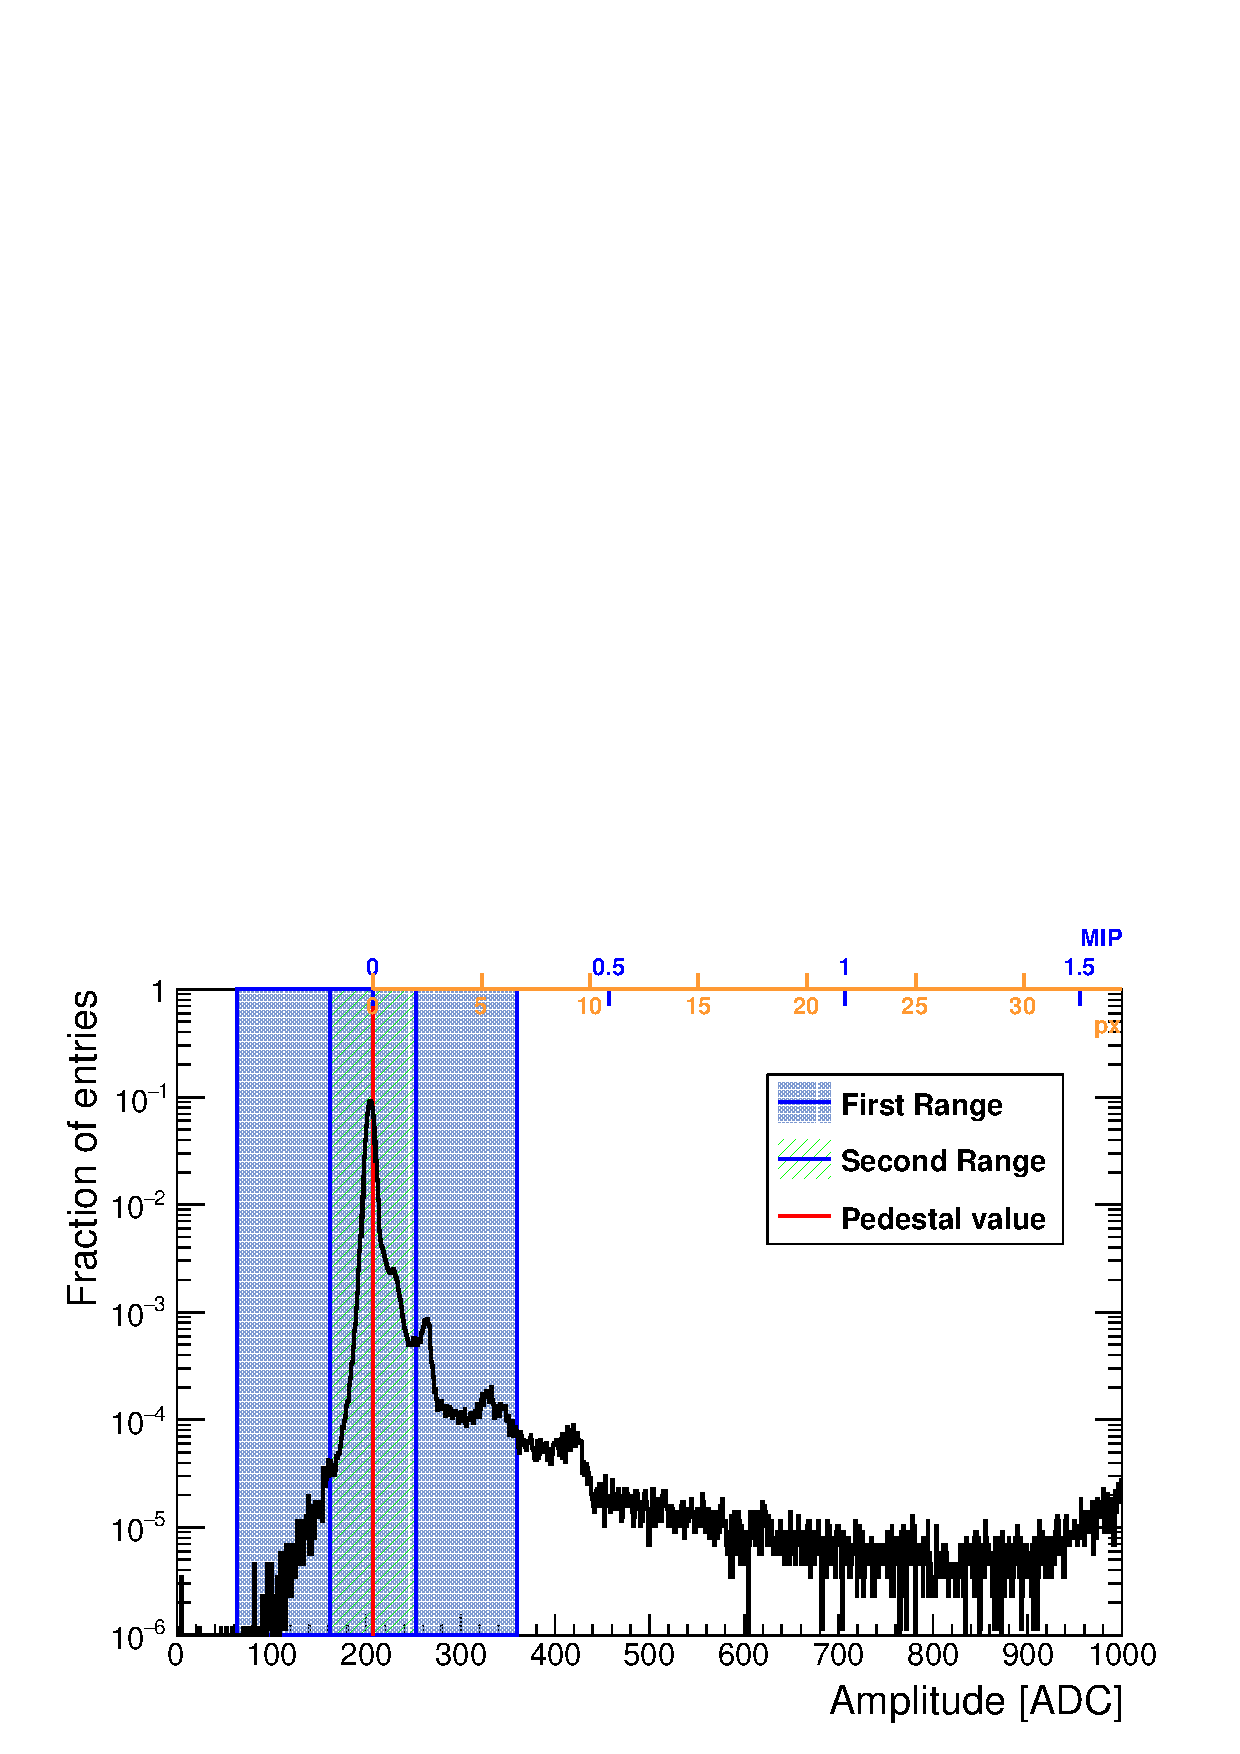
\includegraphics[width=0.6\linewidth]{../Thesis_Plots/EnergyCalib/Plots/PedestalExtractionExample.pdf}
	\caption{Typical pedestal distribution of a channel in auto-trigger mode. The different colored boxed represent the iterative procedure to extract the pedestal value marked with the red line.} \label{fig:PedExtraction}
\end{figure}

As the SiPM noise needs to be taken into account for the pedestal value and considering a Poisson statistic, one to three pixels could be fired due to the dark noise and cross-talk. The fitting range then needs to be in the same order of magnitude of one to three pixels. For this, the histogram range is reduced in the range of 3 RMS around the mean. It is done iteratively two times. Then the mean of the histogram is taken as the pedestal value as shown in figure \ref{fig:PedExtraction}.

As no pedestal subtraction memory cell-wise is performed in the reconstruction at the moment and the CALICE database structure is not designed to have the pedestal constant for each memory cell, a mean over all memory cells is computed per channel. The difference between the mean pedestal and the memory cell wise pedestal is shown in figure \ref{fig:CompMeanMem}. The RMS of the distribution is around 21 ADC which would correspond to an uncertainty of about 4\% on the MIP constant, assuming a typical MIP calibration value of 500 ADC. This error is dominating in the MIP constant uncertainty.

\begin{figure}[htbp!]
	\centering
	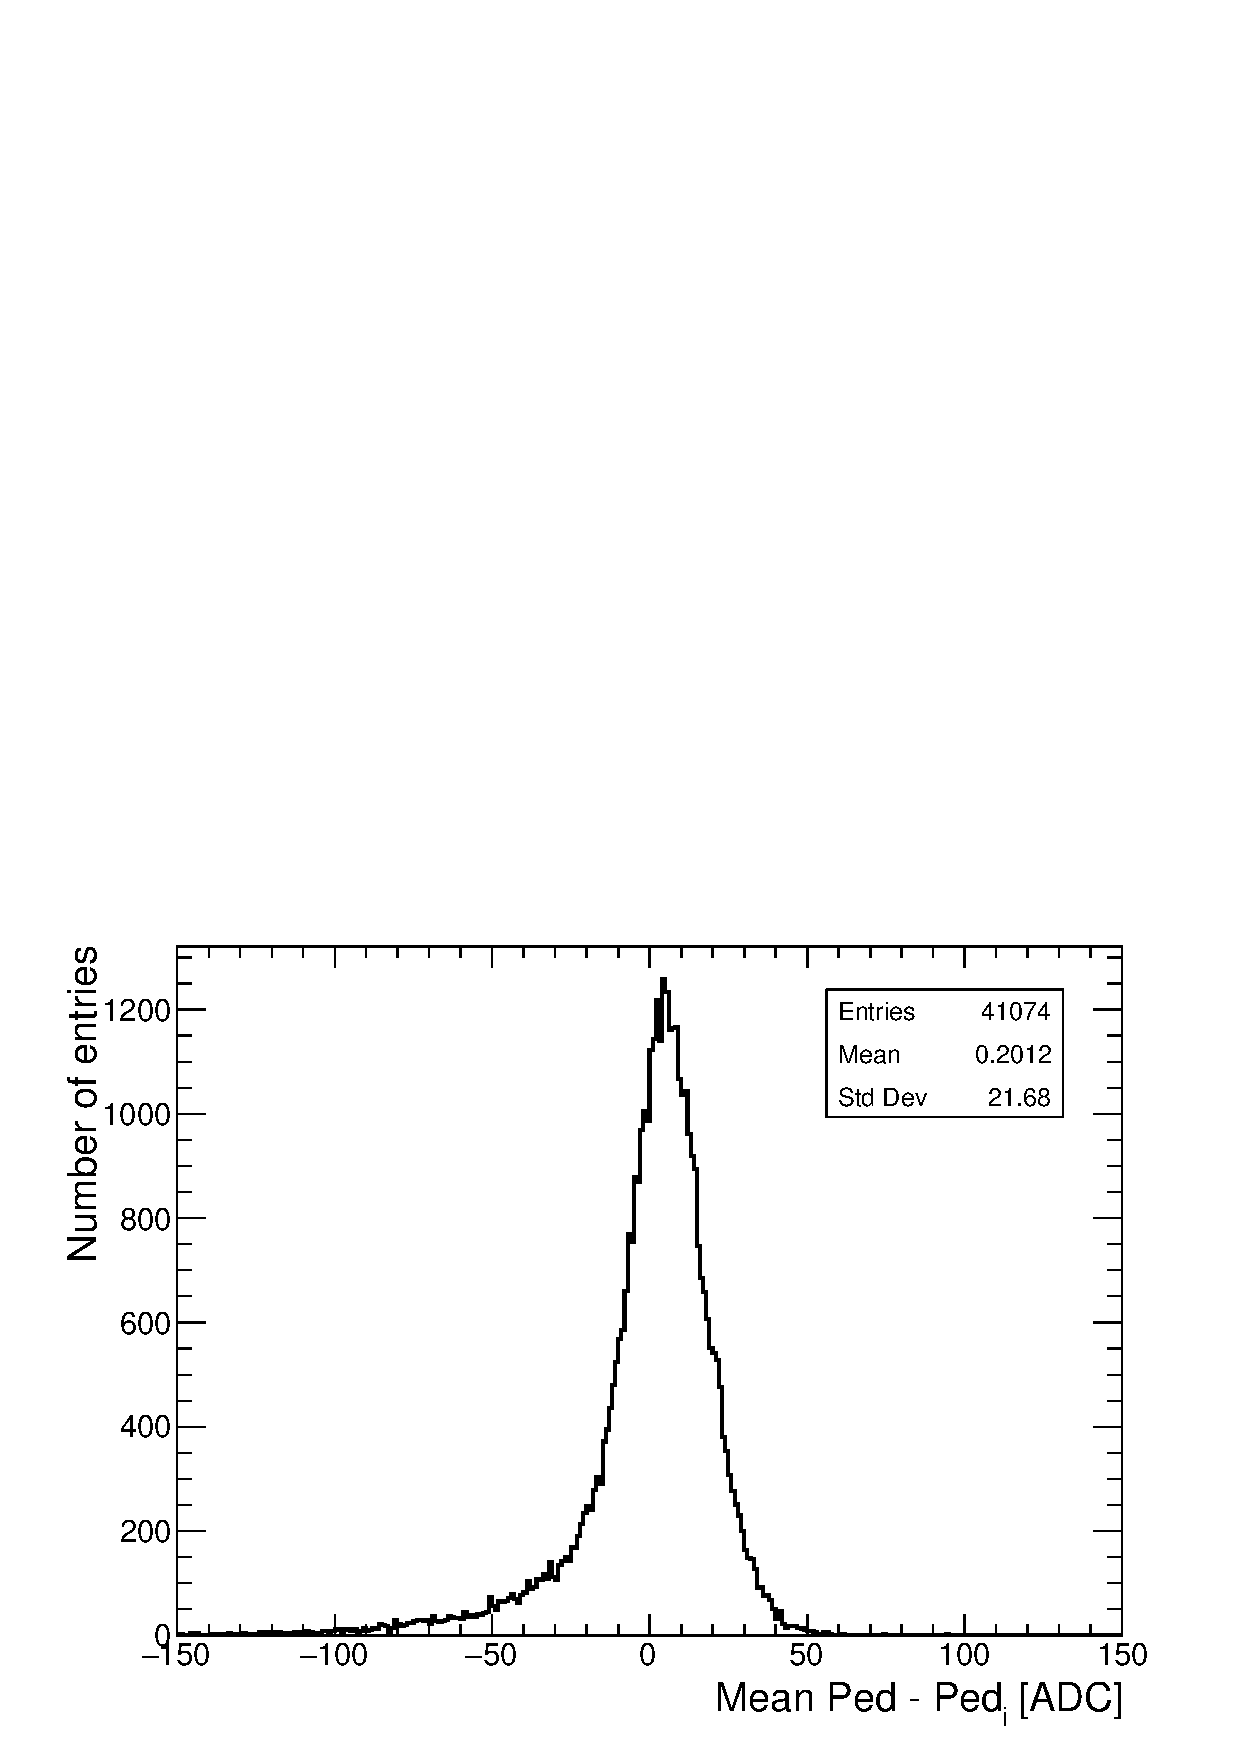
\includegraphics[width=0.6\linewidth]{../Thesis_Plots/EnergyCalib/Plots/ComparisonMeanPedtoMemorycell.pdf}
	\caption{Distribution of the difference between the mean pedestal to the memory-cell wise pedestal per channel.} \label{fig:CompMeanMem}
\end{figure}

\subsection{MIP extraction}
\label{sec:MIPExtraction}

After the pedestal calibration, the extraction of the MIP calibration constant for each channel can be performed. As the detector was equipped with various types of SiPM and boards designs, the extraction procedure needs to be automatic and robust. In order to reduce the amount of noise hits in the hit energy spectra of each cell that would lead to unstable fits and wrong MIP calibration constants, a MIP track selection has been performed as explained in section \ref{subsec:Muon_sel}.

The fitting procedure is very sensitive to the initial parameters of the fit and can be quite difficult with the variety of SiPM and tiles in the AHCAL. To ensure a good fit, an iterative fitting procedure is performed. A more precise and detailed description of the fitting procedure is explained in \cite{FabianThesis}.

Only channels with more than 1000 entries are considered. The parameters in the fit are: the area of the hit energy distribution, the width of the convoluted Gaussian, the most probable value (MPV) of the Landau distribution and the width of the Landau distribution. The spectrum of the hit energy is fitted with a Laudau-Gaussian convolution function for each channel and the maximum of this convoluted function is taken as the MIP constant. A typical example of a single channel fit can be seen in figure \ref{fig:MIPFit}. To ensure a good fit, each channel of the detector have been checked manually.

\begin{figure}[htbp!]
	\centering
	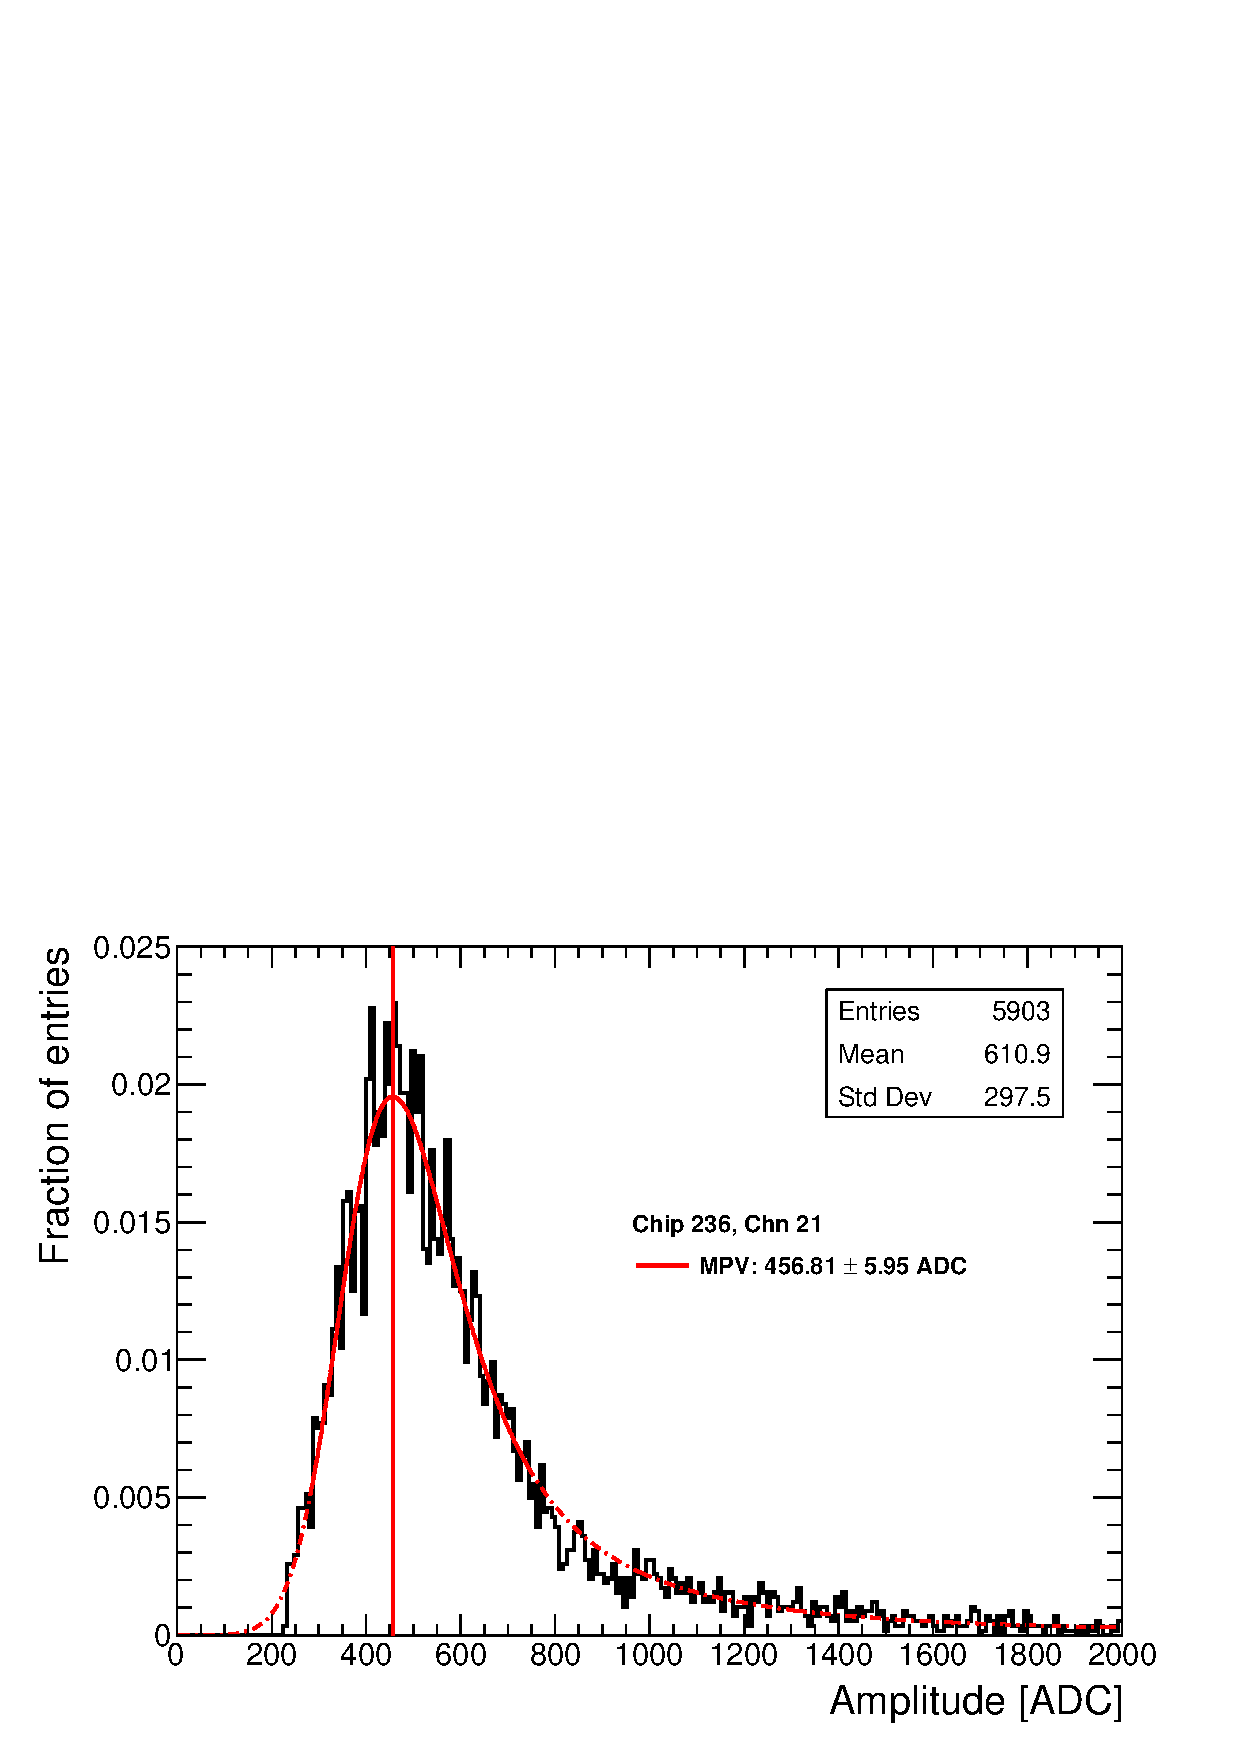
\includegraphics[width=0.6\linewidth]{../Thesis_Plots/EnergyCalib/Plots/ExampleMIP_Module3.pdf}
	\caption{Typical energy distribution in a single channel of the AHCAL with the data collected in July 2015 at CERN. The convoluted function is represented in red with the extracted MIP constant for this channel showed by the vertical red line.} \label{fig:MIPFit}
\end{figure}

\section{Results of the energy scale calibration}

\subsection{MIP extraction results}

Using the muon data recorded in July 2015, 72\% of the channels are fitted over a total number of 3744 channels. This does not mean that 28\% of channels are dead as for the most part, the outer channels (outside of the inner $12\times12$ tiles) of the layers 11 to 14 don't have enough statistics to perform a fit. In order to have a value for the outer channels, especially for the layers 11 to 14, the values are combined with previous testbeams performed in April and May 2015 at DESY with the layers 11 to 14.

Additionally, if a channel is does not have a MIP calibration value, the mean of the MIP constant distribution of a chip or a layer is used. Excluding dead and noisy channels (see appendix \ref{appendix:deadChn}), 3171 channels have been calibrated which accounts for 85\% of the detector channels.

The results of the MIP extraction are shown in table \ref{table:MIPAHCAL} and are regrouped by SiPM types. The results are well compatible with \cite{SarahMaster} although there is slight difference in the number of fitted channels that may come from the differences in the event selection and extraction procedure.

\begin{table}[htb!]
	\centering
	\caption{Table containing the results of the extraction of the MIP calibration constants. The results are regrouped by SiPM type. <MPV> is the mean of the MIP calibration constant distribution per SiPM type. RMS is the standard deviation of MIP calibration constant distribution per SiPM type. Dead and noisy channels are rejected.}
	\label{table:MIPAHCAL}
	\begin{tabular}{@{} lccc @{}}
		\toprule
		Layer \# & <MPV> [ADC] & RMS [ADC] & $N_{fitted}$\\
		\midrule
		1-2 & 66.72 & 35.54 & 172\\
		3 & 501.71 & 50.4 & 142\\
		4-5 & 796.54 & 113.12 & 265\\
		6-10 & 250.99 & 62.72 & 414\\
		11-12 & 285.85 & 62.83 & 1069\\
		13-14 & 307.73 & 58.96 & 1109\\
		\bottomrule
	\end{tabular}
\end{table}

\subsection{Uncertainty of the calibration procedure}

After the calibration, it is necessary to evaluate the uncertainty of the calibration procedure. The figure \ref{fig:MIPError} shows the relative error $\frac{\Delta MIP_i}{MIP_i}$ for all the channels of the detector. The relative error on the MIP calibration value, for most of the channels, is in the expected range of 1\% to 3\% and it is compatible with previous results \cite{SarahMaster}. However, some higher values can be seen due to the layers 1 and 2 where difficulties were met due to a high noise and low SiPM gain.

\begin{figure}[htbp!]
	\centering
	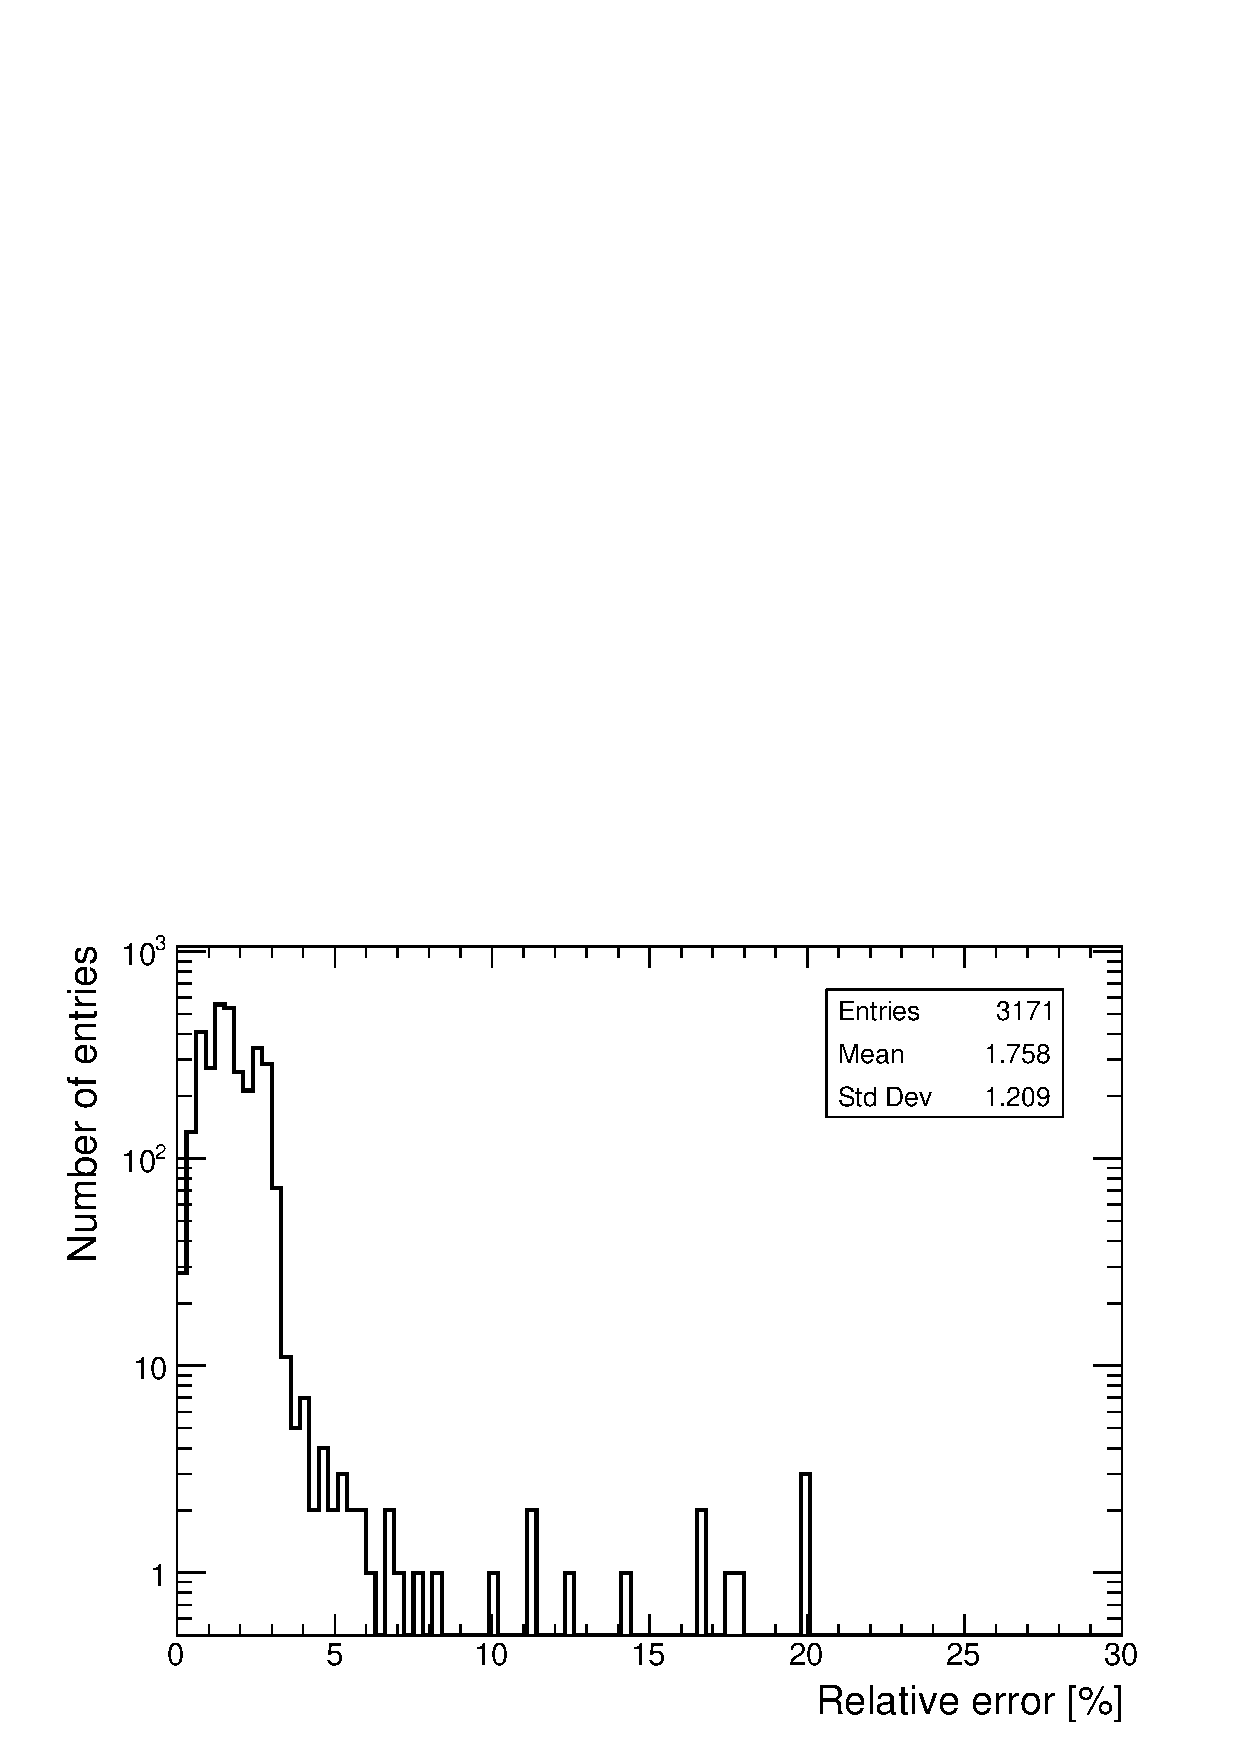
\includegraphics[width=0.6\linewidth]{../Thesis_Plots/EnergyCalib/Plots/RelativeErrorMIP_Combined.pdf}
	\caption{Relative error of the MIP value extracted.} \label{fig:MIPError}
\end{figure}

\subsection{Comparison with simulation}

The MIP calibration defines the energy scale for measuring energy depositions in the AHCAL. It is needed to carefully calibrate and validate the MIP calibration in data and simulation in order to get comparable results. Applying the MIP selection, it results in energy depositions of single MIP amplitudes for all channels. The comparison of the MIP spectrum for the whole AHCAL between data and simulation in figure \ref{fig:MIPData_MC} shows that the shape of the hit energy spectrum matches relatively well. The data appears slightly wider than for simulation as channel-wise mis-calibrations are not modeled in the simulation. This comparison validates the digitization of scintillator-SiPM readout calorimeters.

\begin{figure}[htbp!]
	\begin{subfigure}[t]{0.5\textwidth}
		\centering
		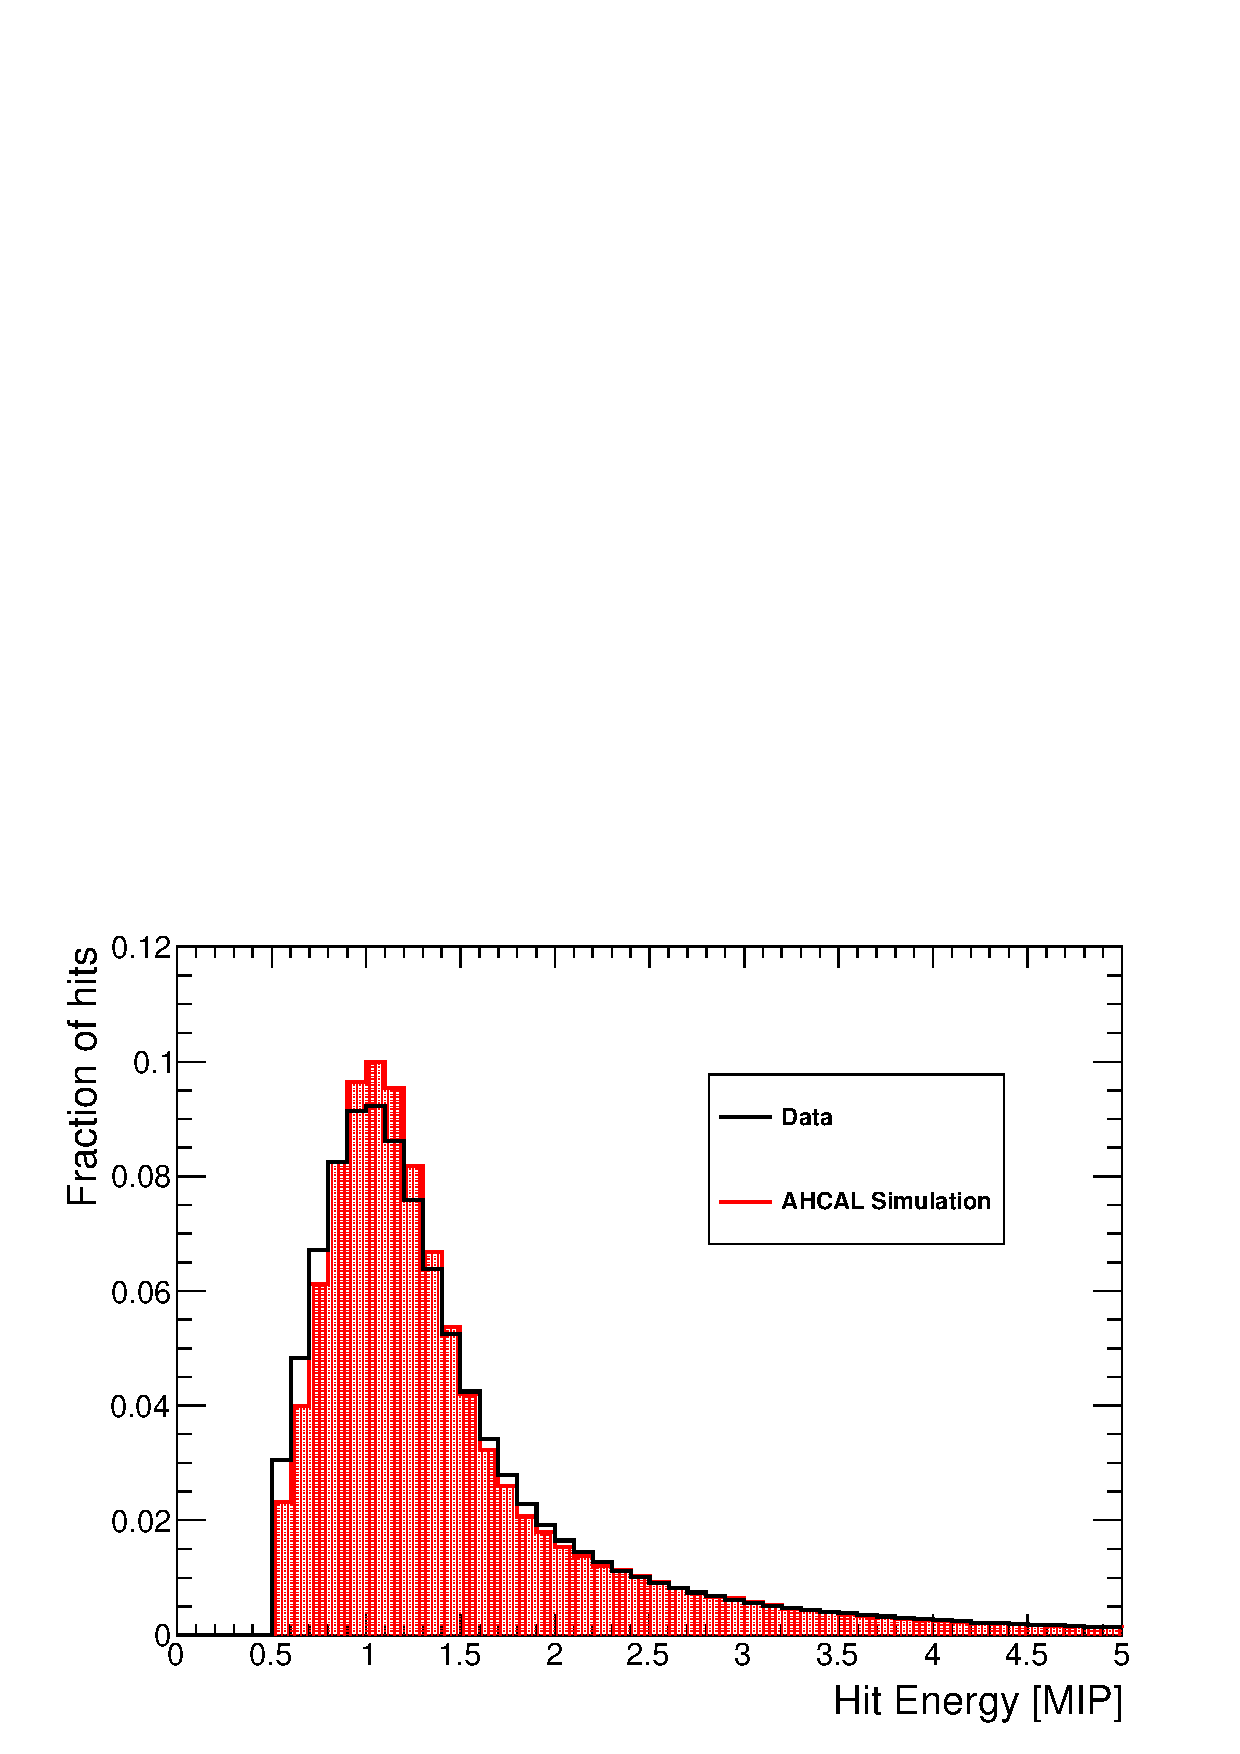
\includegraphics[width=1\linewidth]{../Thesis_Plots/EnergyCalib/Plots/ComparisonMCData_MIPPeak.pdf}
		\caption{} \label{fig:MIPData_MC}
	\end{subfigure}
	\hfill
	\begin{subfigure}[t]{0.5\textwidth}
		\centering
		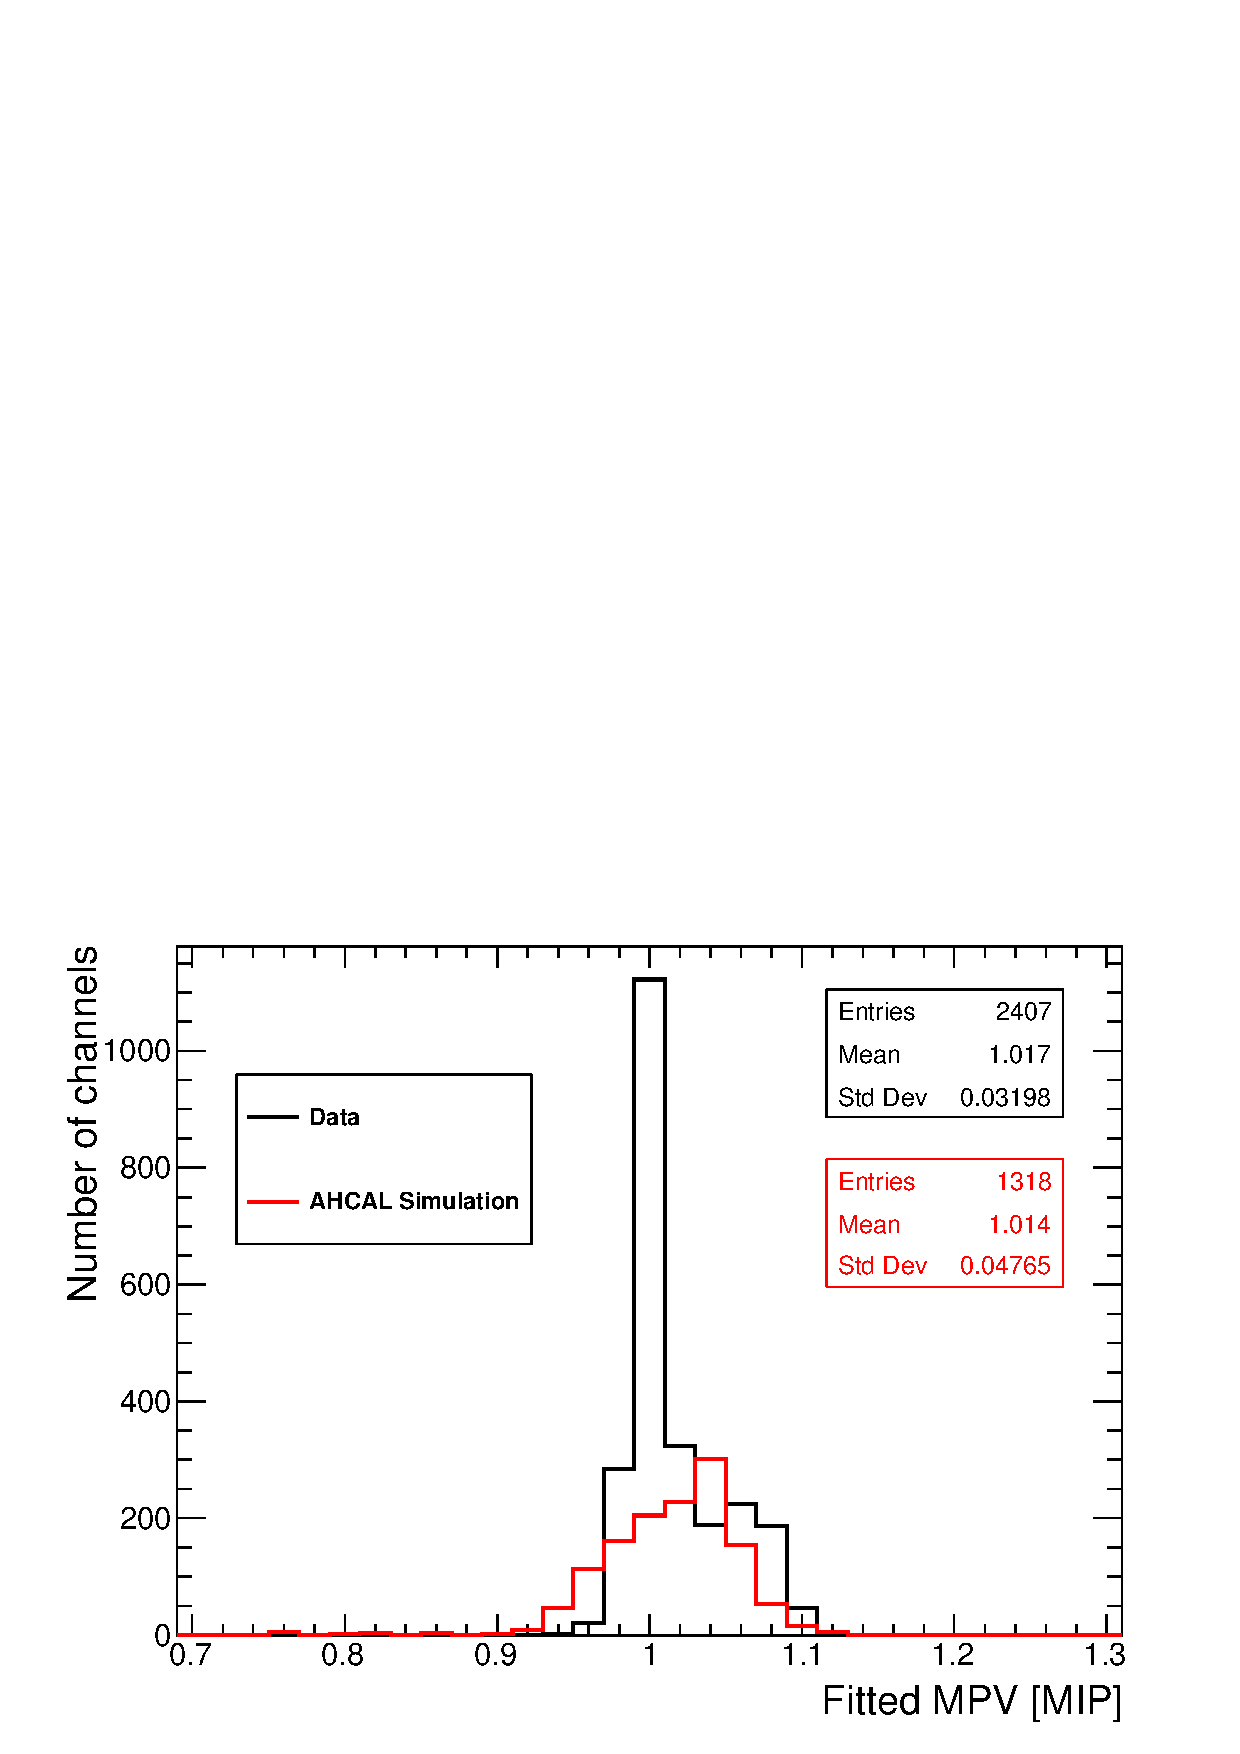
\includegraphics[width=1\linewidth]{../Thesis_Plots/EnergyCalib/Plots/ComparisonMCData_MPV.pdf}
		\caption{} \label{fig:MPVData_MC}
	\end{subfigure}
	\caption{\subref{fig:MIPData_MC}) Hit Energy Spectra for the complete AHCAL for muon like-track hits in the data of July 2015 for both data and simulation. \subref{fig:MPVData_MC}) Distribution of fitted MPV in single channels of the AHCAL for both data and simulation.}
\end{figure}

The extraction of the MIP calibration value in data and simulation has been done for each single channels of the AHCAL. The figure \ref{fig:MPVData_MC} shows the distribution of the extracted MIP calibration constant for single channels in both data and simulation. Ideally, the distribution should peak at the unity for all channels. But in practice, due to the fitting procedure uncertainty, mis-calibrations and statistic limitation, it results in a widening of the distribution. Both data and simulation give a mean value around 1 MIP for the AHCAL indicating a good average calibration at the cell level. The higher values to the right that appear in the data have been checked and all channels present a good fit. The AHCAL simulation is slightly shifted to the right to higher values but still reasonably close to unity.

\subsection{Systematic on the MIP scale}

A systematic error on the MIP energy scale can be derived by dividing the data muon sample into two sub-samples by even or odd run number. This will take into account not only the uncertainty on the MIP calibration but as well temperature variations and temporal variations. Then each sample is fitted using the same fitting procedure as described in section \ref{sec:MIPExtraction}. This systematic uncertainty can then be used in the timing analysis described in the next chapters.

\begin{figure}[htbp!]
	\centering
	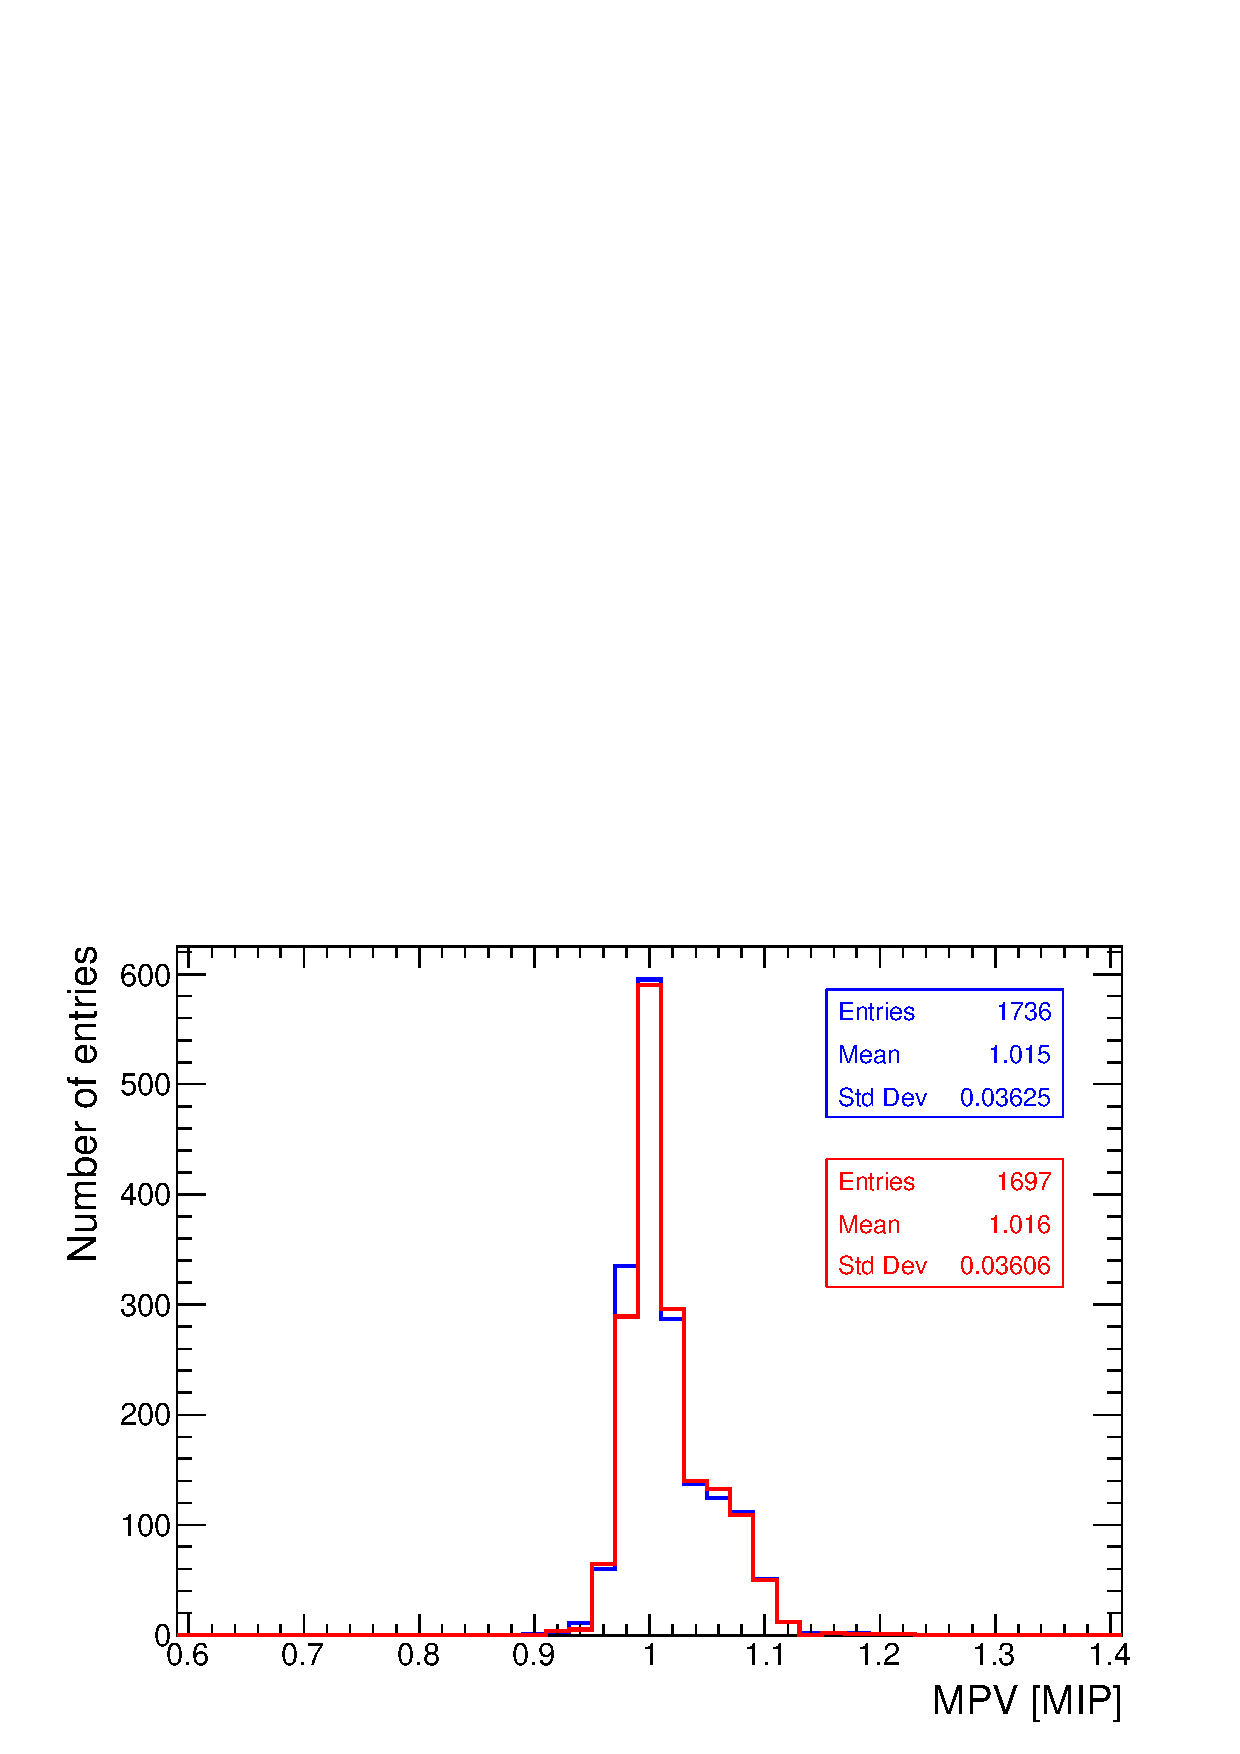
\includegraphics[width=0.7\linewidth]{../Thesis_Plots/EnergyCalib/Plots/SystematicMIP.pdf}
	\caption{MPV fitted value in MIP for the two muon sub-samples. Even runs are in blue, odd runs are in red.} \label{fig:MIPSyst}
\end{figure}

Both samples are very similar with a shift in the mean value of less than 1\%. As previously seen, a slight shoulder is present to higher MIP values though the mean is still very close to unity. By looking at the mean of the RMS of both distributions, a systematic uncertainty of around 3.6\% on the MIP energy scale can be derived.

\section{Validation studies}
\label{appendix:SimulationVal}

Once the energy scale calibration of the AHCAL has been performed, a validation of the simulation model can be done in order to be able to compare the recorded data and simulation in a latter stage.
In this section, an extensive validation of the simulation is shown. The AHCAL simulation model is validated by comparing electromagnetic shower observables in data and simulation. Electromagnetic interactions within the AHCAL are used as these interactions should be well described in simulations and are less subject to modeling uncertainties.

\section{Beam profiles}

The simulation needs as one input the position and width of the particle gun. It has to be placed in x, y directions such that the beam sizes of the experiment are modeled and in order to guaranty that the same cells of the detector are hit in the simulation as in data. Otherwise, dead and noisy channels could bias the comparison between data and simulation. In the z-direction, the beam gun needs to be put as close as possible to the detector to avoid beam broadening by scattering on air molecules.

The best method to estimate the beam profile for data would be to analyze the beam profile provided by the wired chambers. Unfortunately, this data is not available for this analysis. As a workaround, the mean and RMS of the center of gravity distributions in x and y are used to estimate the beam size instead. This does not reflect the true positions since both positions are biased by dead and noisy channels. This has been done for electrons runs as well as for pions runs for each energy. No significant differences in beam profile are visible on a run-by-run basis. The muon beam is simulated by a plane square distribution with a half-width of 20 cm. The center of gravity is calculated as the following:

\begin{equation}
  CoG_x [mm] = \frac{\Sigma_i E_i x_i}{\Sigma_i E_i} \quad \text{,} \quad CoG_y [mm] = \frac{\Sigma_i E_i y_i}{\Sigma_i E_i} \quad \text{and} \quad CoG_z [mm] = \frac{\Sigma_i E_i z_i}{\Sigma_i E_i}
\end{equation}

\noindent with $E_i$ the energy of the i-th hit and $x_i$ and $y_i$ the x and y position of the i-th hit.

The beam profiles in the x and y directions for muons are shown in figures \ref{fig:BPmu} for data and simulation. The beam profile is not perfectly reproduced but is good enough. This will have a slight impact on the data and simulation comparison as we are very sensitive to the
profile of the beam.

\begin{figure}[htbp!]
  \centering
  \begin{subfigure}[t]{0.49\textwidth}
    \includegraphics[width=1.\linewidth]{../Thesis_Plots/Timing/Muons/Plots/BeamProfileX.pdf}
    \caption{CoG X.} \label{fig:mu150GeVX}
  \end{subfigure}
  \hfill
  \begin{subfigure}[t]{0.49\textwidth}
    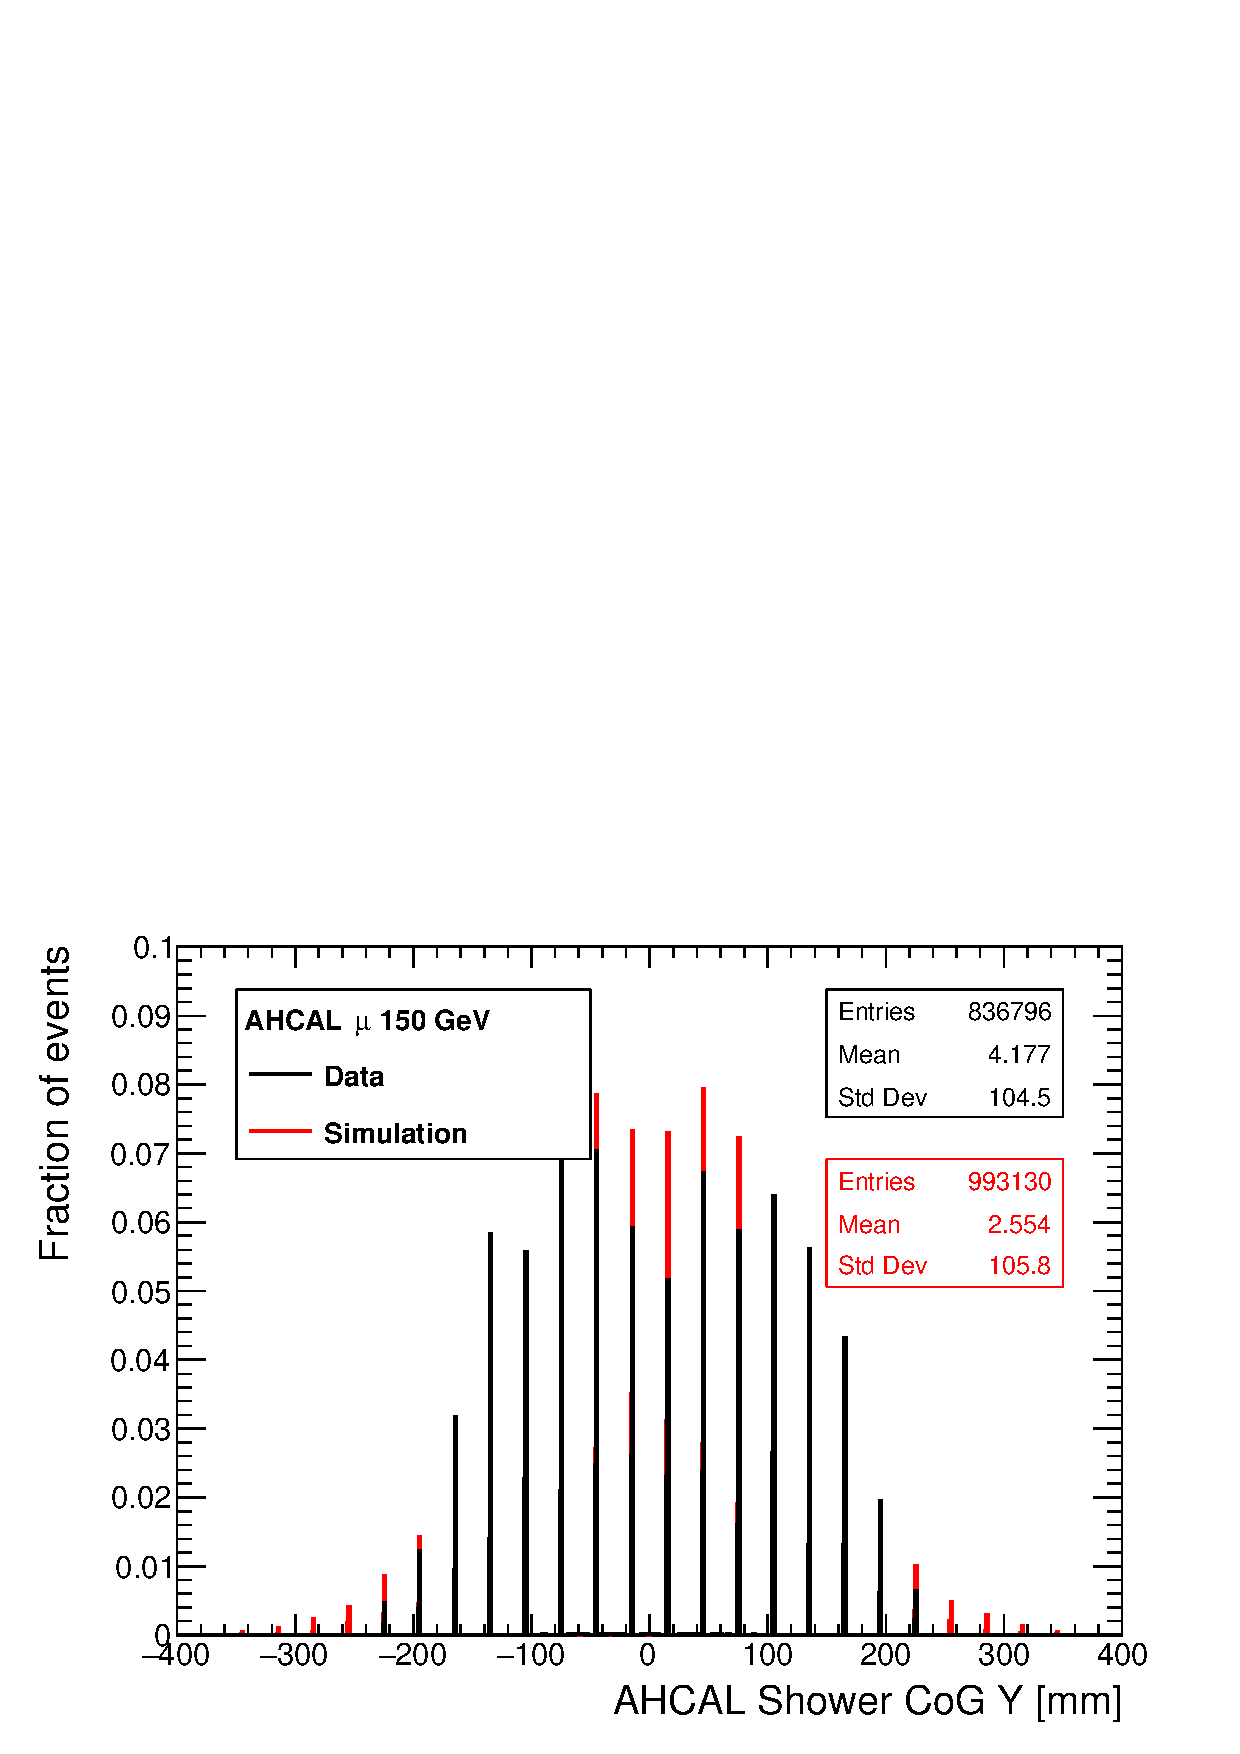
\includegraphics[width=1.\linewidth]{../Thesis_Plots/Timing/Muons/Plots/BeamProfileY.pdf}
    \caption{CoG Y.} \label{fig:mu150GeVY}
  \end{subfigure}
  \caption{Beam profiles for 150 GeV muons for data and simulation in the x and y directions.}
  \label{fig:BPmu}
\end{figure}

Figures \ref{fig:BPe} show the beam profiles in the x and y directions for data and simulation for 10 GeV and 50 GeV electrons. The agreement looks much better for 10 GeV than for 50 GeV, this may be due to contamination from lower energy electrons. Moreover, at higher energy, the beam looks less gaussian-like and the shape in simulation can't be simulated correctly. Figures \ref{fig:BPpi} show the beam profiles in the x and y-direction for data and simulation for 10 GeV and 90 GeV pions. The agreement looks quite good for both energies in the x-direction, only a slight difference is visible in the y-direction but should have not much impact.

\begin{figure}[htbp!]
  \centering
  \begin{subfigure}[t]{0.49\textwidth}
    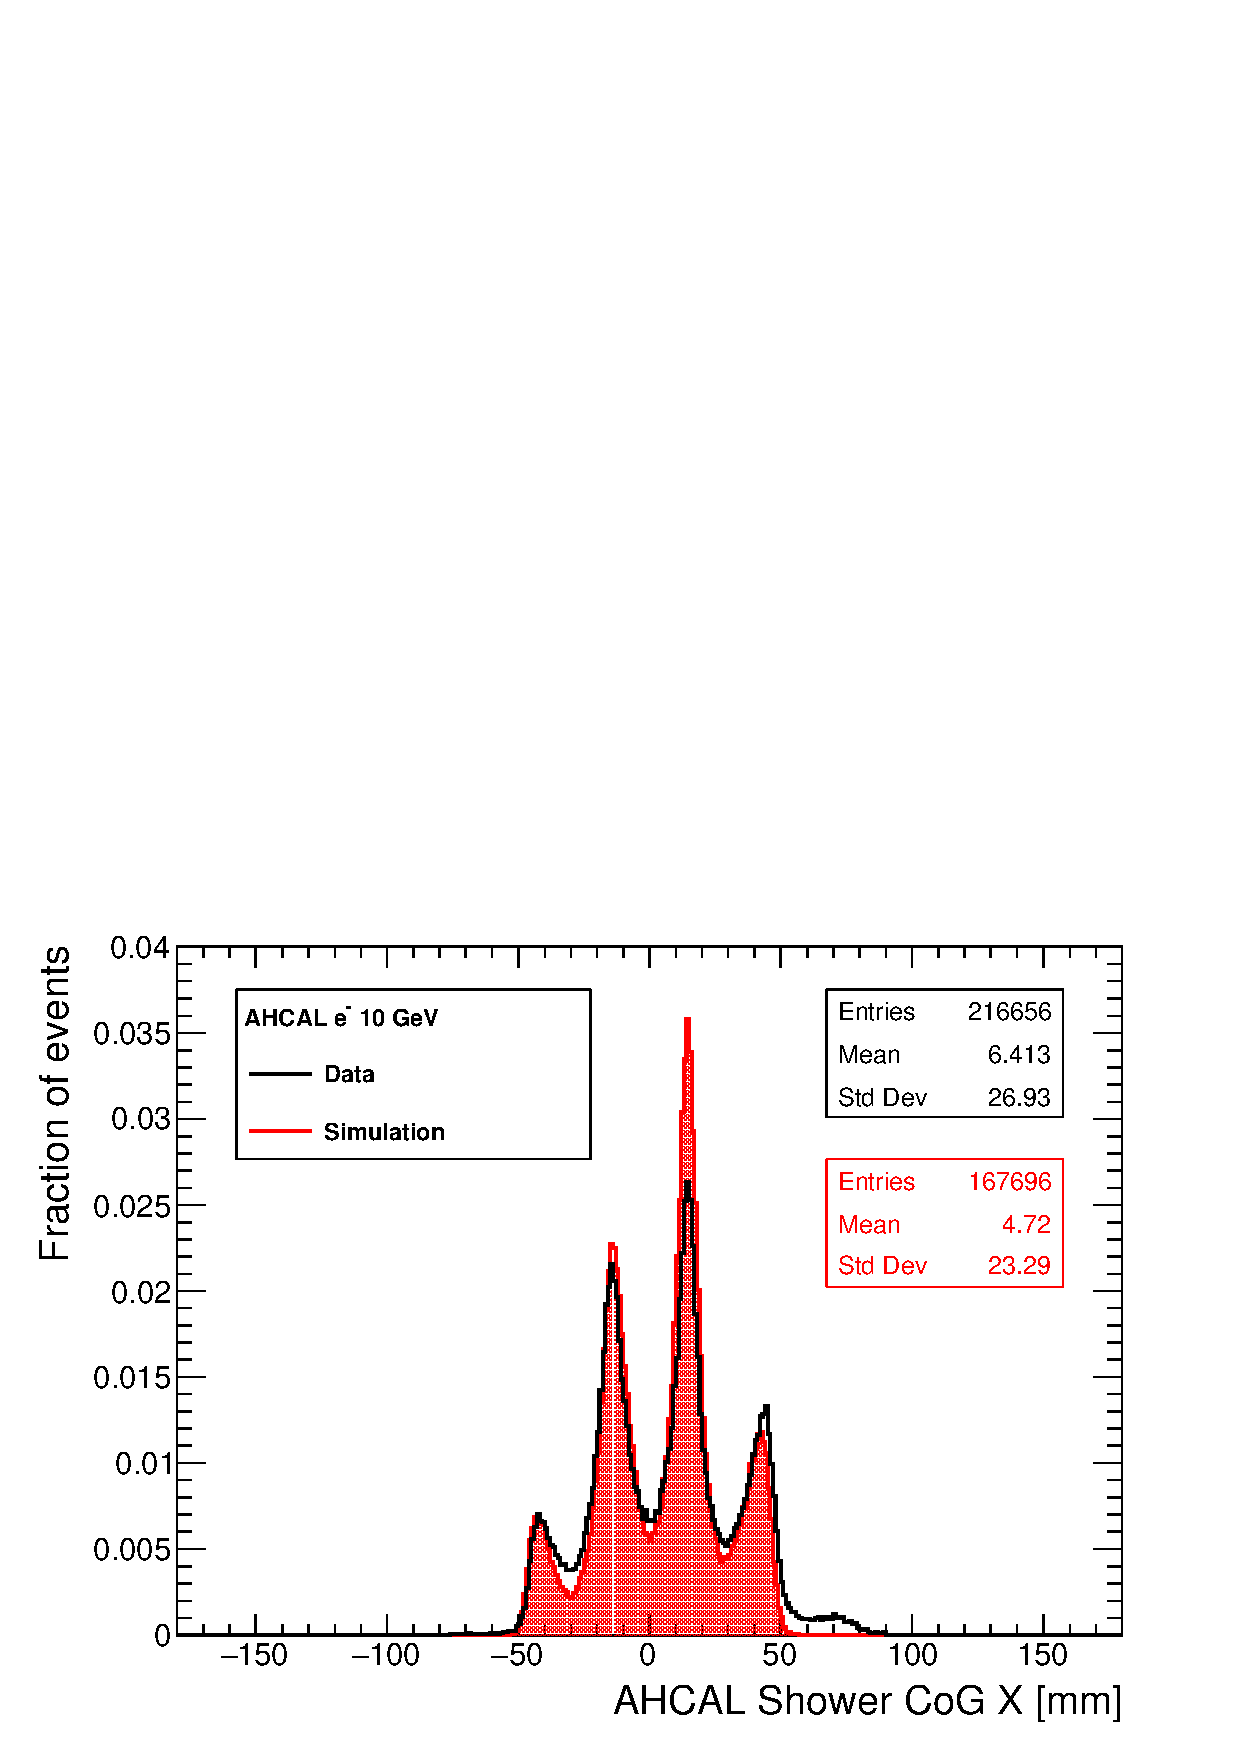
\includegraphics[width=1.\linewidth]{../Thesis_Plots/Timing/Electrons/Plots/Run24542_CoGX_AHCAL_10GeV_Comparison.pdf}
    \caption{10 GeV.} \label{fig:e10GeVX}
  \end{subfigure}
  \hfill
  \begin{subfigure}[t]{0.49\textwidth}
    \includegraphics[width=1.\linewidth]{../Thesis_Plots/Timing/Electrons/Plots/Run24542_CoGY_AHCAL_10GeV_Comparison.pdf}
    \caption{10 GeV.} \label{fig:e10GeVY}
  \end{subfigure}
  \hfill
  \begin{subfigure}[t]{0.49\textwidth}
    \includegraphics[width=1.\linewidth]{../Thesis_Plots/Timing/Electrons/Plots/Run24405_CoGX_AHCAL_50GeV_Comparison.pdf}
    \caption{50 GeV.} \label{fig:e50GeVX}
  \end{subfigure}
  \hfill
  \begin{subfigure}[t]{0.49\textwidth}
    \includegraphics[width=1.\linewidth]{../Thesis_Plots/Timing/Electrons/Plots/Run24405_CoGY_AHCAL_50GeV_Comparison.pdf}
    \caption{50 GeV.} \label{fig:e50GeVY}
  \end{subfigure}
  \caption{Beam profiles for 10 GeV and 50 GeV electrons for data and simulation in the x and y directions.}
  \label{fig:BPe}
\end{figure}

\begin{figure}[htbp!]
  \centering
  \begin{subfigure}[t]{0.49\textwidth}
    \includegraphics[width=1.\linewidth]{../Thesis_Plots/Timing/Pions/Plots/Run24306_CoGX_AHCAL_10GeV_Comparison.pdf}
    \caption{10 GeV.} \label{fig:pi10GeVX}
  \end{subfigure}
  \hfill
  \begin{subfigure}[t]{0.49\textwidth}
    \includegraphics[width=1.\linewidth]{../Thesis_Plots/Timing/Pions/Plots/Run24306_CoGY_AHCAL_10GeV_Comparison.pdf}
    \caption{10 GeV.} \label{fig:pi10GeVY}
  \end{subfigure}
  \hfill
  \begin{subfigure}[t]{0.49\textwidth}
    \includegraphics[width=1.\linewidth]{../Thesis_Plots/Timing/Pions/Plots/Run24332_CoGX_AHCAL_90GeV_Comparison.pdf}
    \caption{90 GeV.} \label{fig:pi90GeVX}
  \end{subfigure}
  \hfill
  \begin{subfigure}[t]{0.49\textwidth}
    \includegraphics[width=1.\linewidth]{../Thesis_Plots/Timing/Pions/Plots/Run24332_CoGY_AHCAL_90GeV_Comparison.pdf}
    \caption{90 GeV.} \label{fig:pi90GeVY}
  \end{subfigure}
  \caption{Beam profiles for 10 GeV and 90 GeV pions for data and simulation in the x and y directions.}
  \label{fig:BPpi}
\end{figure}

\section{Validation of the simulation model}

\subsection{Muons}

In order to justify any comparison made with the simulation, it needs to be validated first. This is done in two steps using muons and electrons. The comparison of the energy deposited and the number of hits in data and simulation is used to validate the detector simulation. Figures \ref{fig:muVal} show the visible energy $E_{sum}$ and the number of hits above 0.5 MIP for 150 GeV muons in data and simulation.

\begin{figure}[htbp!]
  \centering
  \begin{subfigure}[t]{0.49\textwidth}
    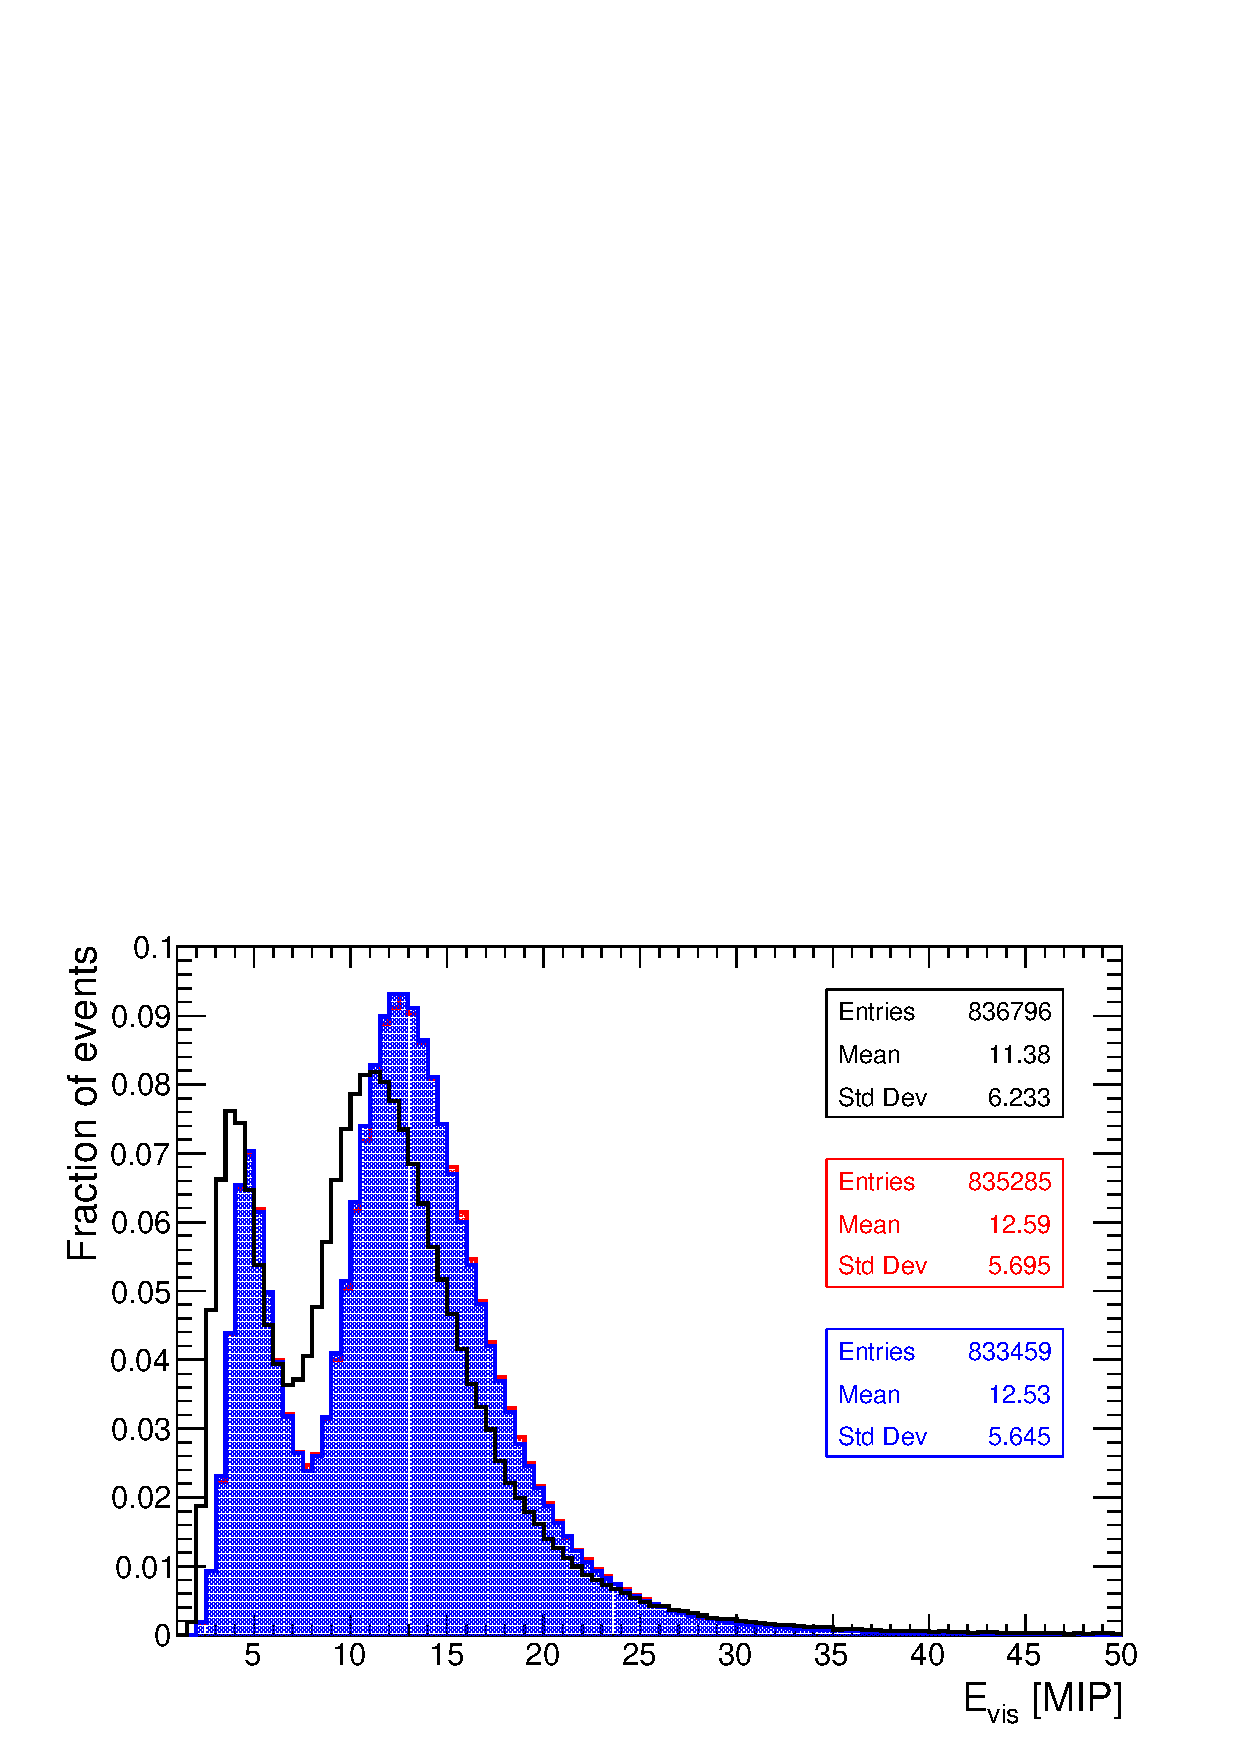
\includegraphics[width=1.\linewidth]{../Thesis_Plots/Timing/Muons/Plots/Validation_Evis_Muons.pdf}
    \caption{$E_{sum}$.} \label{fig:muEvis}
  \end{subfigure}
  \hfill
  \begin{subfigure}[t]{0.49\textwidth}
    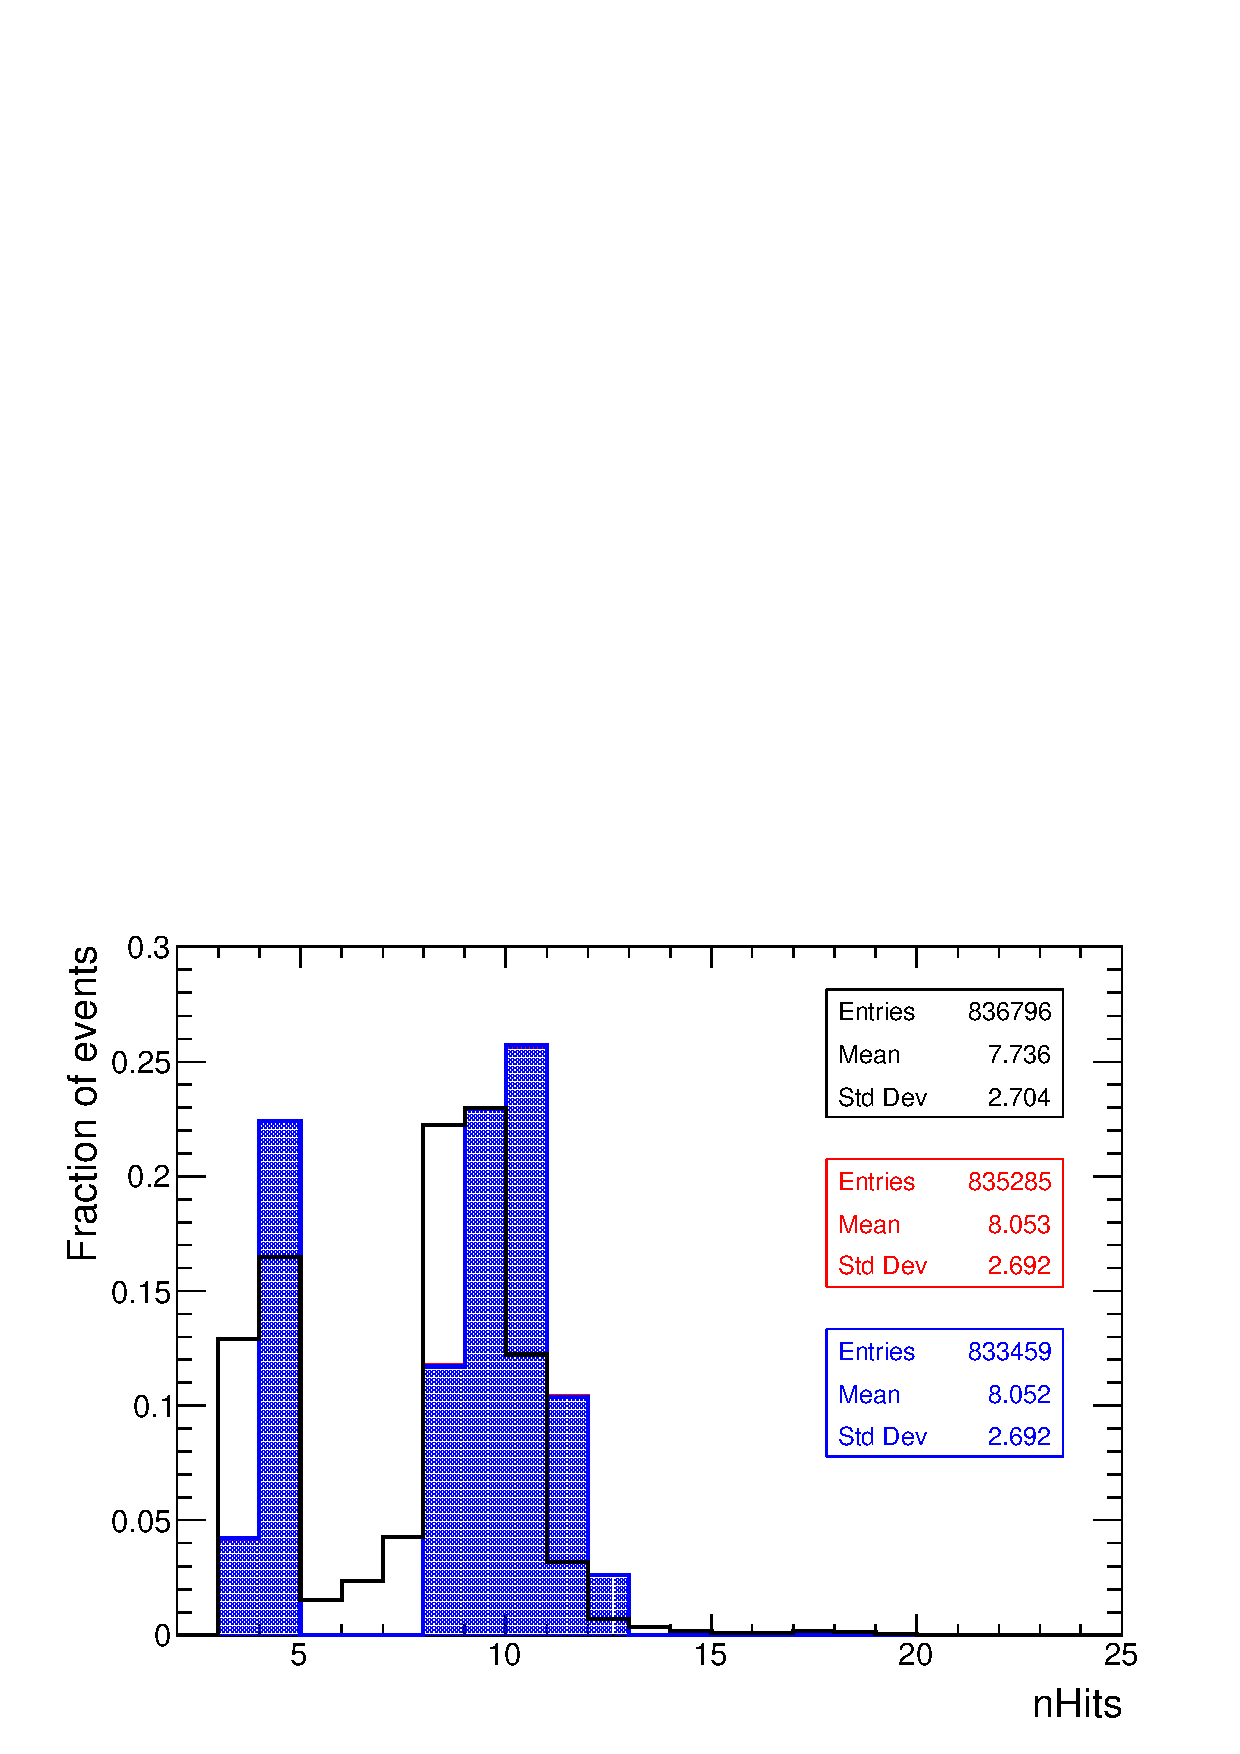
\includegraphics[width=1.\linewidth]{../Thesis_Plots/Timing/Muons/Plots/Validation_nHits_Muons.pdf}
    \caption{nHits.} \label{fig:munHits}
  \end{subfigure}
  \caption{\subref{fig:muEvis}) The energy sum in the AHCAL for 150 GeV muons in data and simulations. \subref{fig:munHits}) The number of hits in the AHCAL for 150 GeV muons in data and simulations.}
  \label{fig:muVal}
\end{figure}

One can notice that the distributions are quite similar though the simulation shows a higher mean deposited energy and also fewer entries to around 5 MIP. As well simulation seems to show a slightly higher number of hits. This may be due to the beam profile that is not perfectly well reproduced in the simulation. In this case, the impact of dead channels is high depending on where the beam is located. Further, an investigation of the energy deposited per layer has been done and can be seen in figure \ref{fig:muEdep}. It shows that the simulations agree with the data within 5\%. This indicates that the calibration has been performed well for all layers.

\begin{figure}[htbp!]
  \centering
  \begin{subfigure}[t]{0.49\textwidth}
    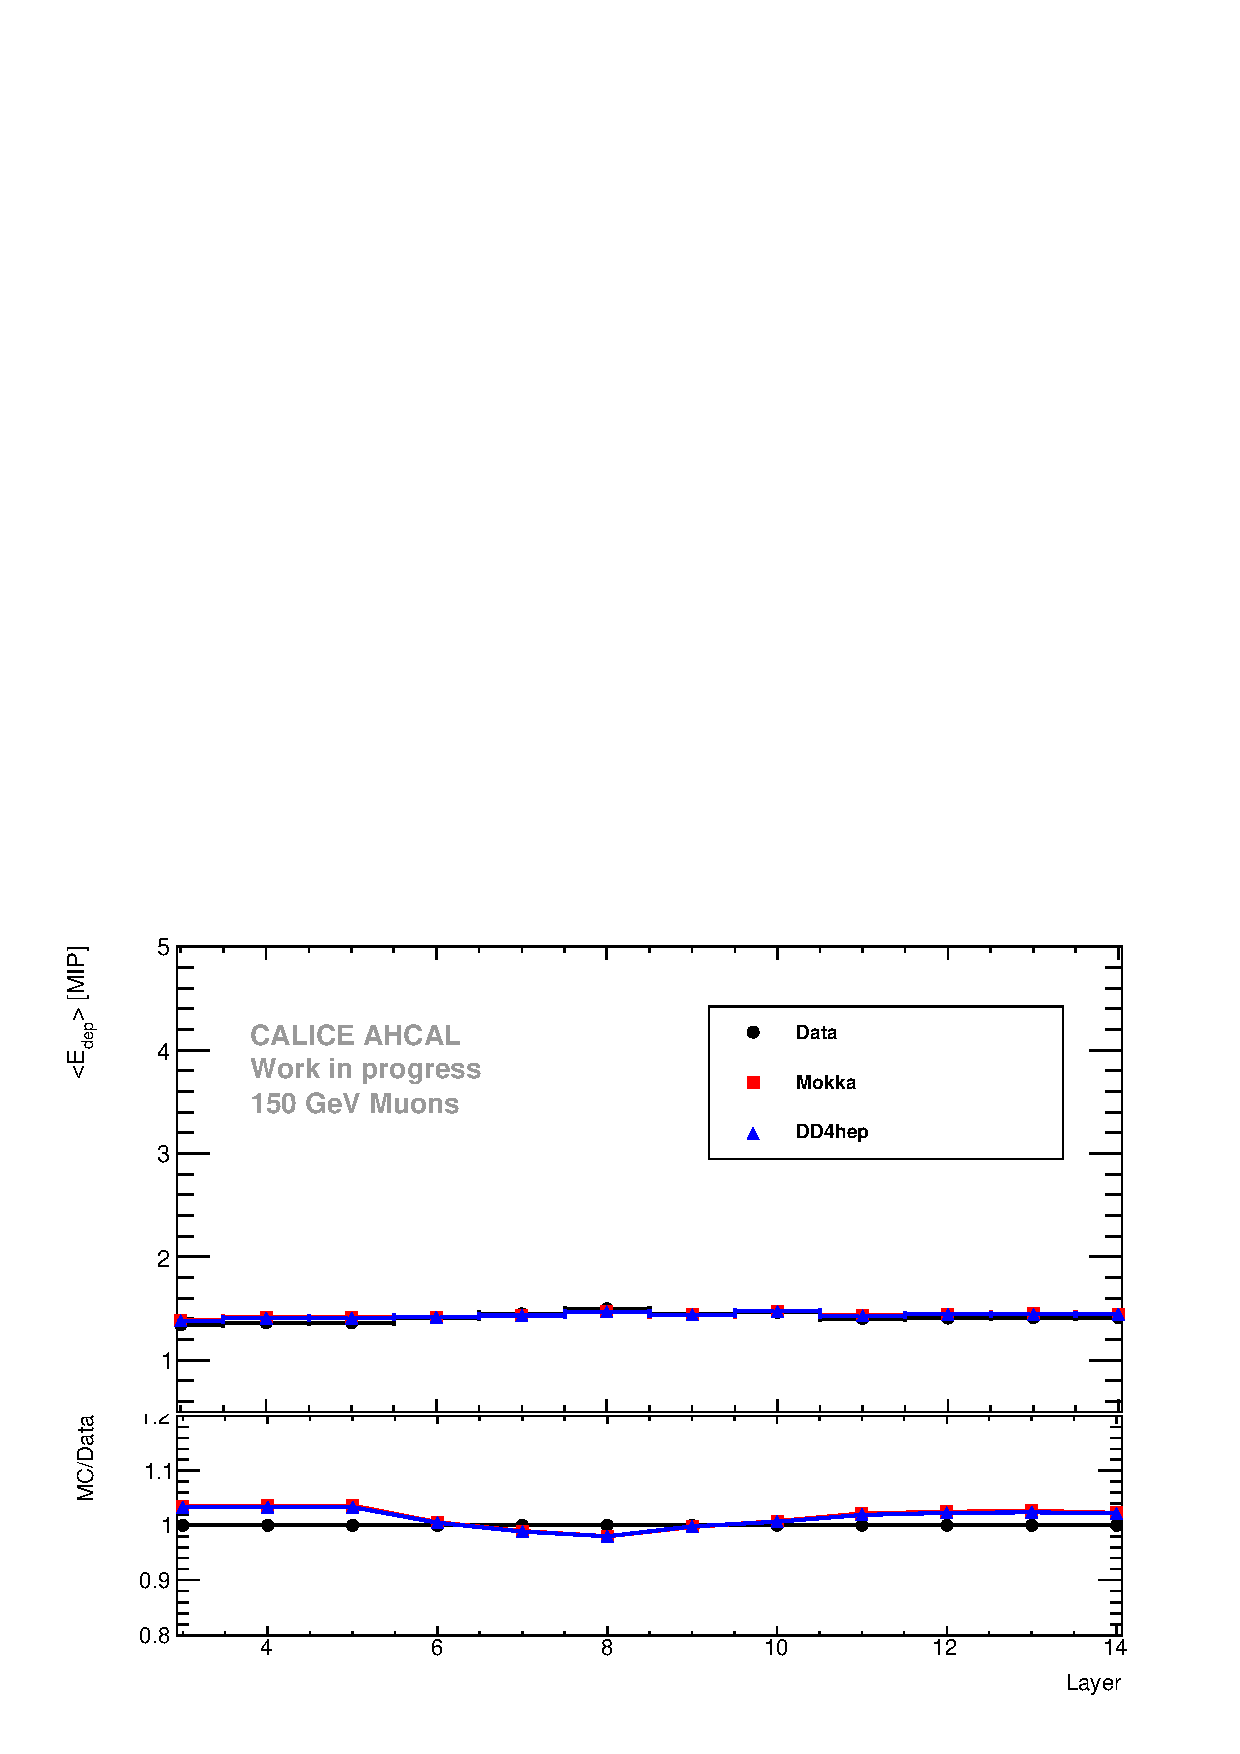
\includegraphics[width=1\linewidth]{../Thesis_Plots/Timing/Muons/Plots/ProfileMuons_Edep.pdf}
    \caption{} \label{fig:muEdep}
  \end{subfigure}
  \hfill
  \begin{subfigure}[t]{0.49\textwidth}
    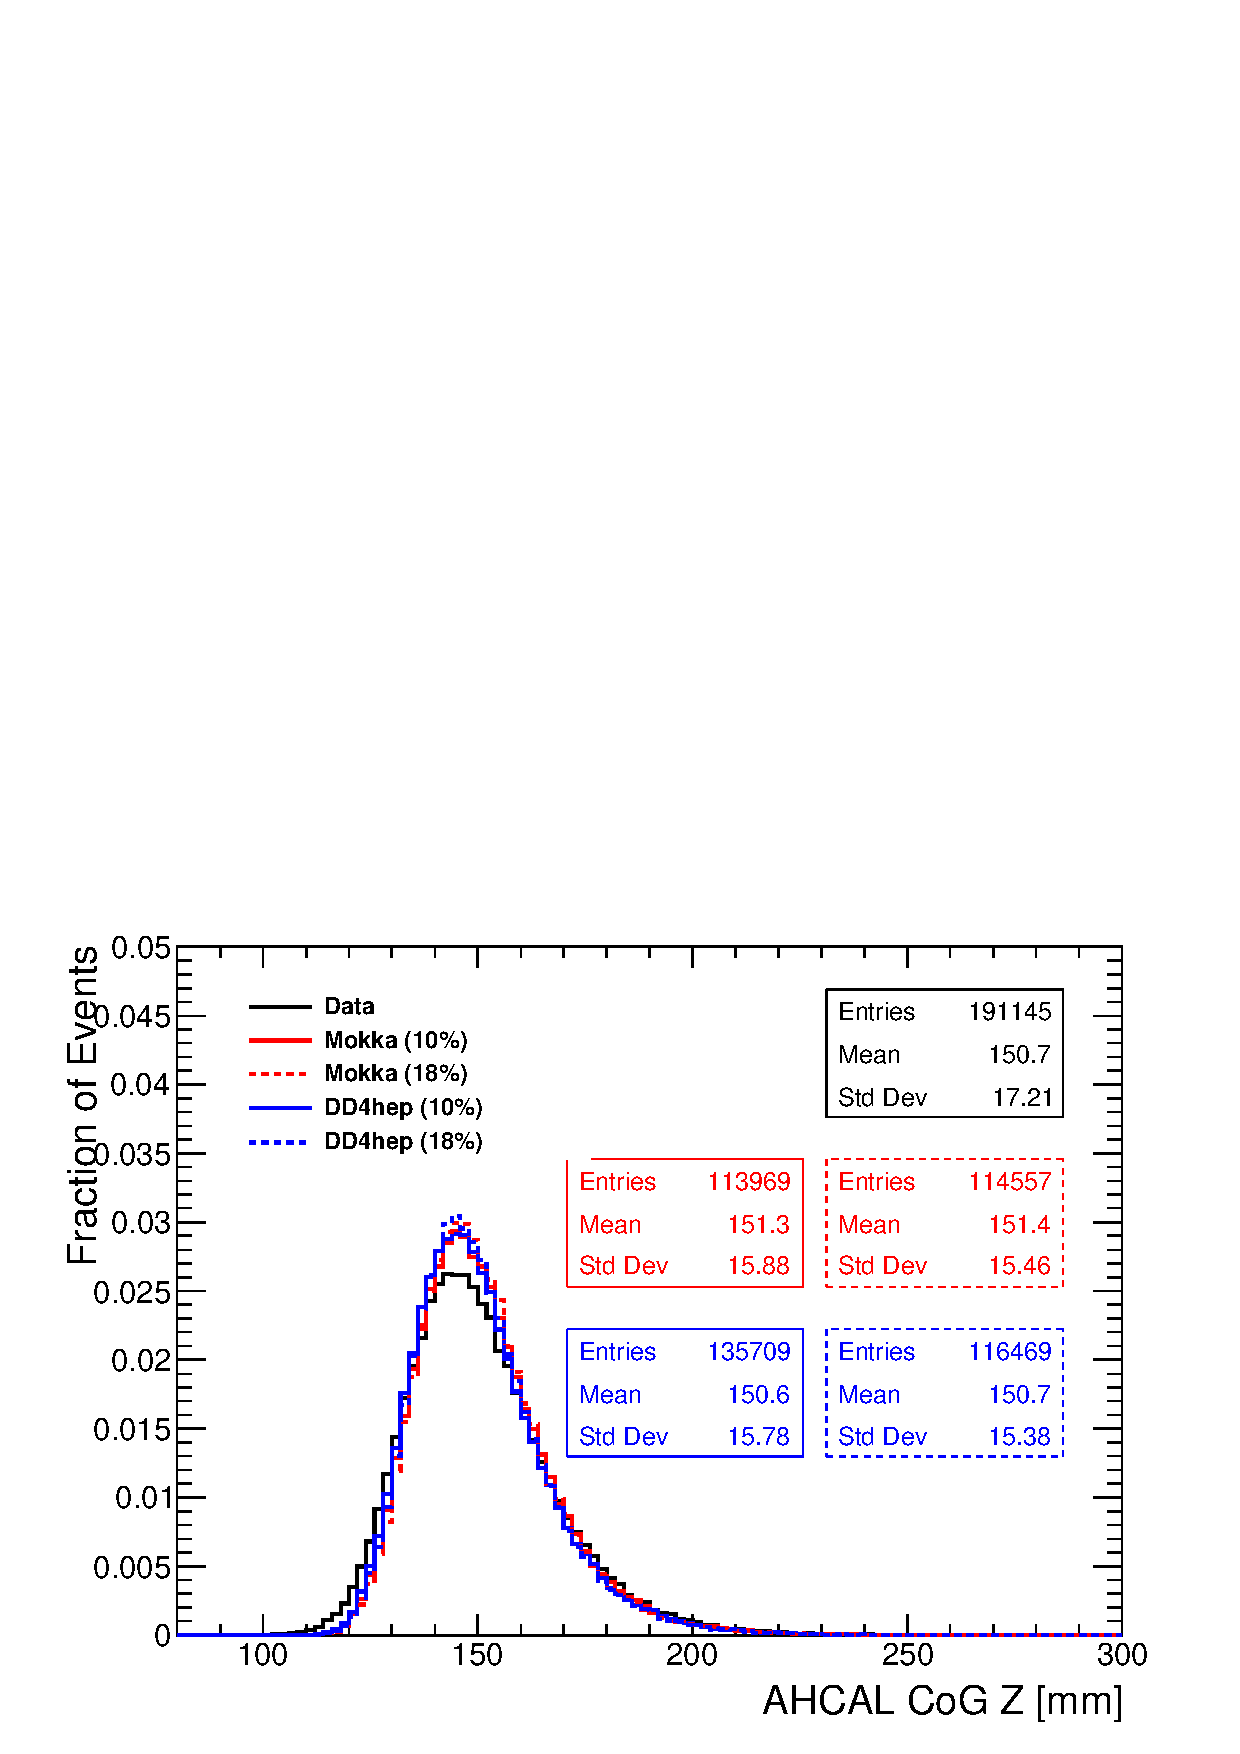
\includegraphics[width=1.\linewidth]{../Thesis_Plots/Timing/Electrons/Plots/Comparison_CoGZ_Xtalk_electrons10GeV.pdf}
    \caption{} \label{fig:e10GoGZ}
  \end{subfigure}
  \caption{\subref{fig:muEdep}) Longitudinal energy profile for 150 GeV muons for data and simulations. \subref{fig:e10GoGZ}) Distribution of the center of gravity in the z direction for 10 GeV electrons for data and simulation.}
  \label{fig:Val}
\end{figure}

\subsection{Electrons}

In a second part, electrons are used to validate further the simulation. As the physics of electron showers are very well understood and can be simulated with great accuracy, it is used as a tool to validate the detector geometry, especially concerning the material budget. Also besides noise and beam profiles, the influence of cross-talk has a significant impact due to the higher energy deposited. Moreover, desaturation of high energy cells is very important as generally electrons deposit in few cells their energy. Unfortunately, no saturation curves are available and only estimations of the necessary parameters are derived from simulation by tuning it to the data. Though, in this analysis, the energy deposited in a single cell is only relevant at low energies (from 0.5 to few MIPs) where the response of the SiPM is linear. Thus desaturation is not used. On the other side, only saturation of the hit energy is performed on the simulation where the same parameters are used, this has an effect on the matching between data and simulations for the energy sum but similar as the desaturation does not matter for this analysis. Simple shower variables have been looked at such as the number of hits, energy sum and center of gravity in z-direction per event in order to validate the simulation.

The center of gravity in z was looked at as this variable is most sensible to the amount of material upstream to the calorimeter. The figure \ref{fig:e10GoGZ} shows that the data and simulations agree rather well despite the data seems to shower slightly before. Figures \ref{fig:e10Val} and \ref{fig:e50Val} show the distribution of the energy sum $E_{sum}$ in the AHCAL and the number of hits $nHits$ for 10 GeV and 50 GeV electrons for data and simulations. Two different version of the simulations, with a cross-talk parameter of 10\% or 18\% are shown. For 10 GeV, 10\% cross-talk seems better whereas, for 50 GeV, the value of 18\% seems favored. A value of 15\% was chosen for the simulation as neither simulations fit the data for both observables. One can also notice that for 50 GeV, a large tail to the left of both distributions is visible. This has been investigated in details \cite{AmbraEnergy}, but the origin of this is still not clear and may come from contamination from lower energy electrons. This is not a problem in itself for this analysis as only timing is investigated.

\begin{figure}[htbp!]
  \centering
  \begin{subfigure}[t]{0.49\textwidth}
    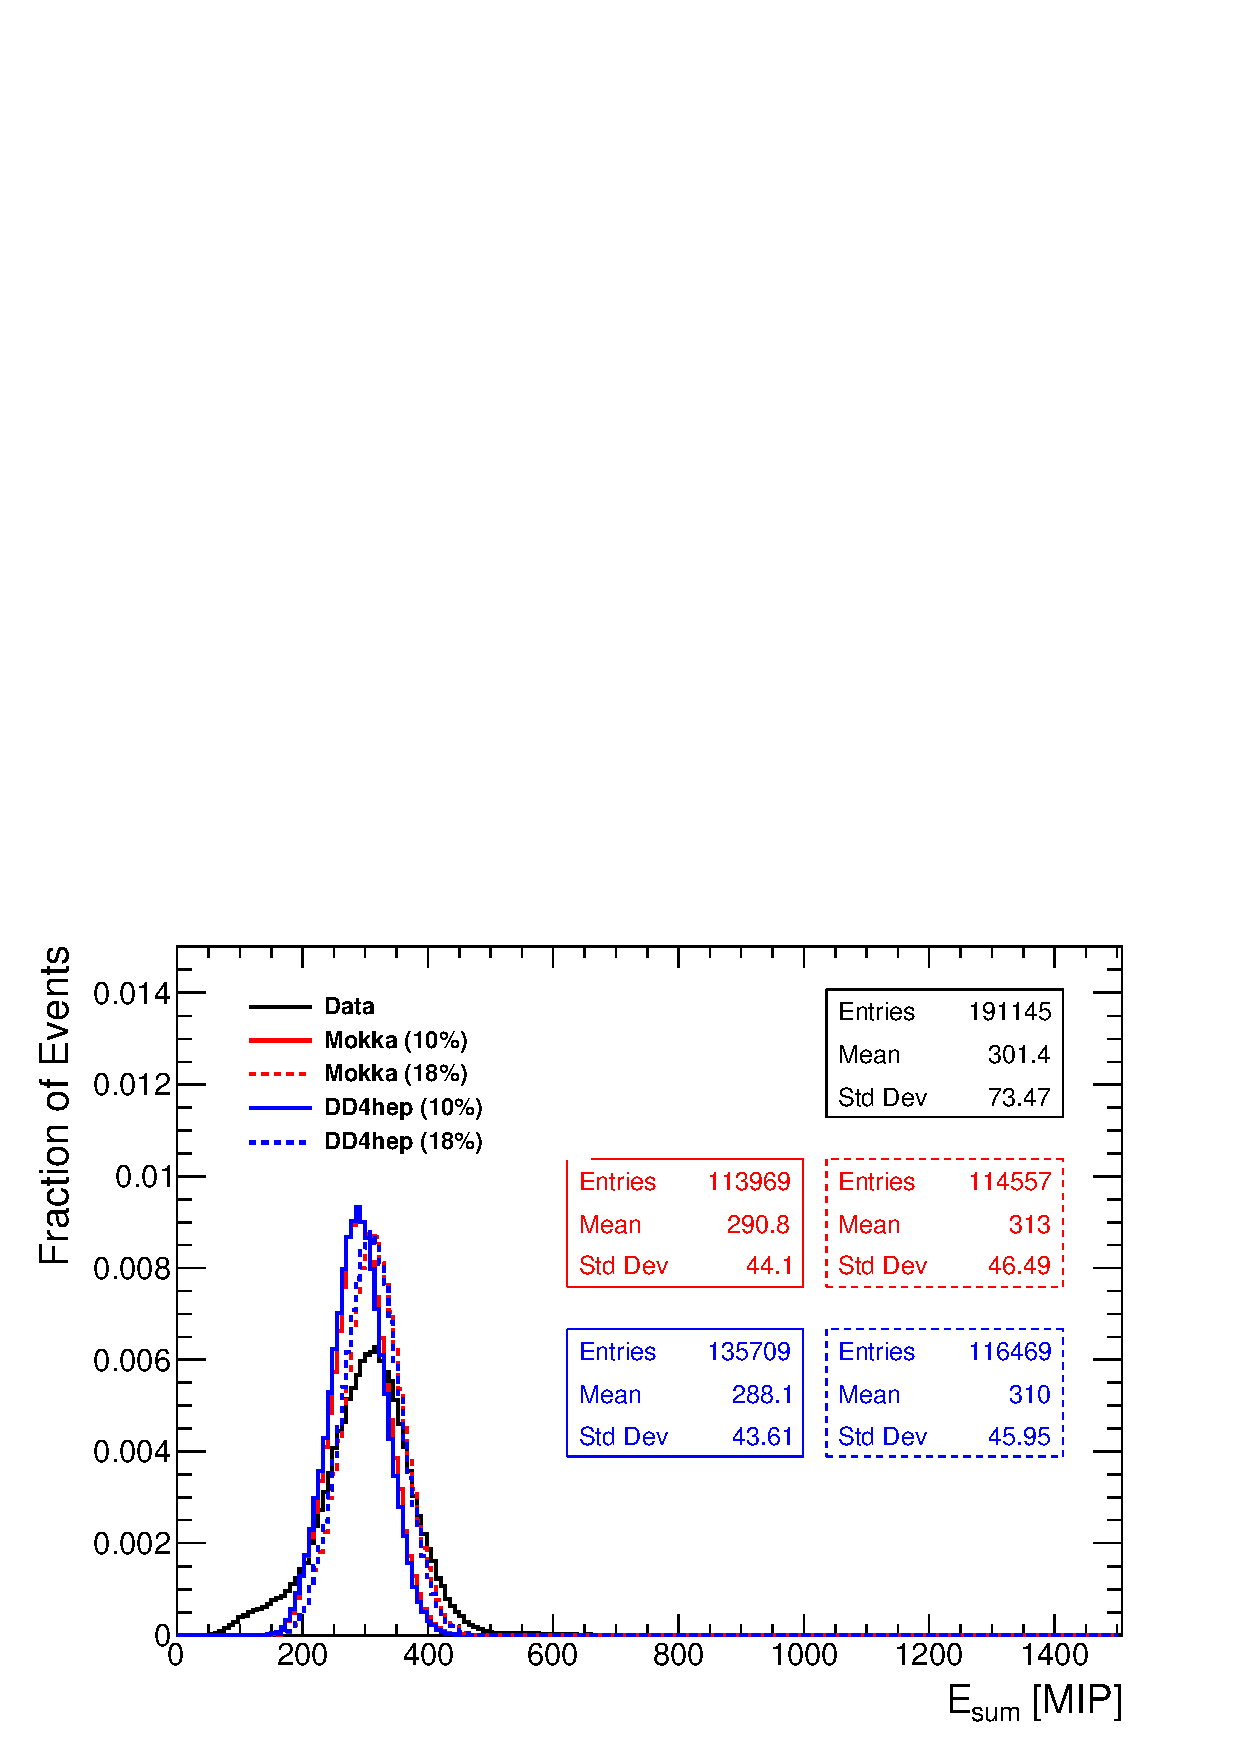
\includegraphics[width=1.\linewidth]{../Thesis_Plots/Timing/Electrons/Plots/Comparison_EnergySum_Xtalk_electrons10GeV.pdf}
    \caption{$E_{sum}$.} \label{fig:e10Evis}
  \end{subfigure}
  \hfill
  \begin{subfigure}[t]{0.49\textwidth}
    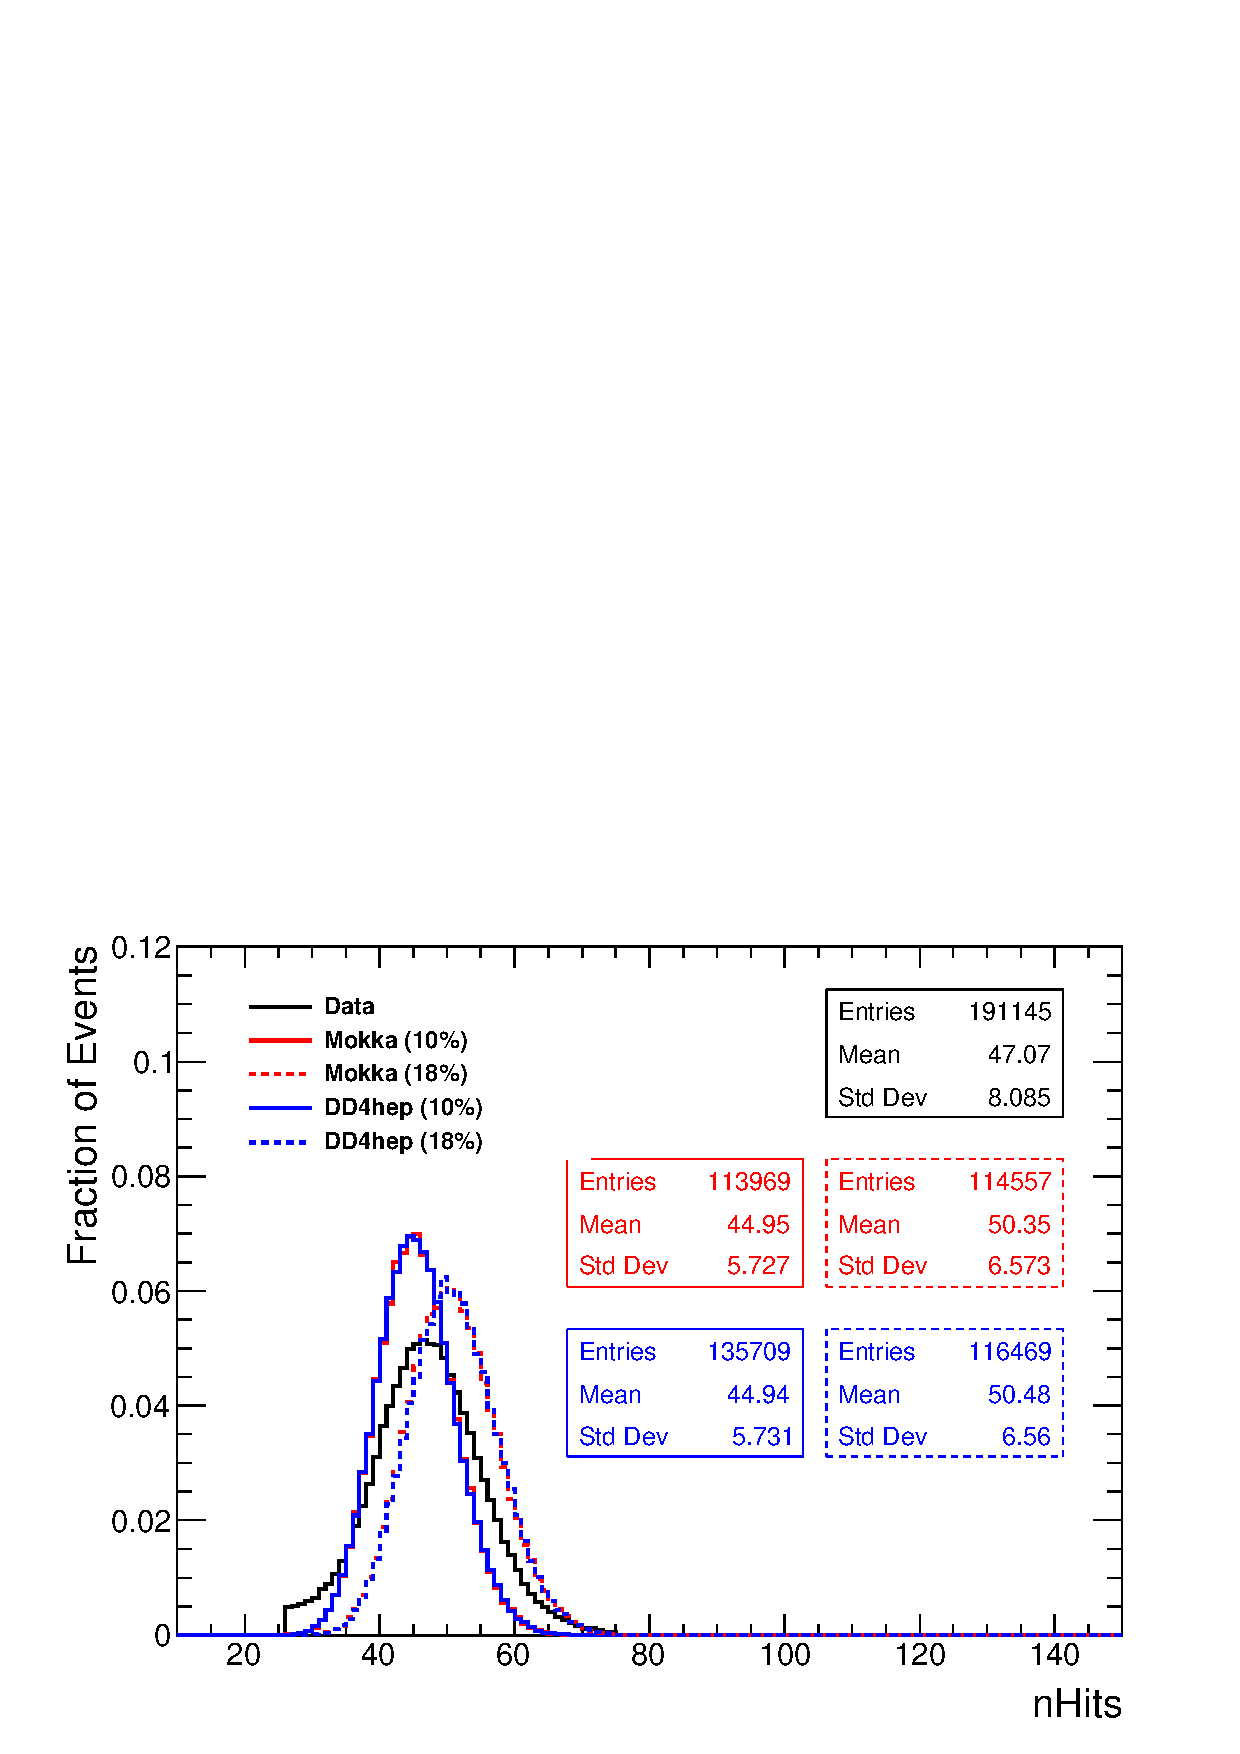
\includegraphics[width=1.\linewidth]{../Thesis_Plots/Timing/Electrons/Plots/Comparison_nHits_Xtalk_electrons10GeV.pdf}
    \caption{nHits.} \label{fig:e10nHits}
  \end{subfigure}
  \caption{\subref{fig:e10Evis}) The energy sum in the AHCAL for 10 GeV electrons for data and simulations with a cross-talk value of 10\% and 18\%. \subref{fig:e10nHits}) The number of hits in the AHCAL for 10 GeV electrons for data and simulations with a cross-talk value of 10\% and 18\%.}
  \label{fig:e10Val}
\end{figure}

\begin{figure}[htbp!]
  \centering
  \begin{subfigure}[t]{0.49\textwidth}
    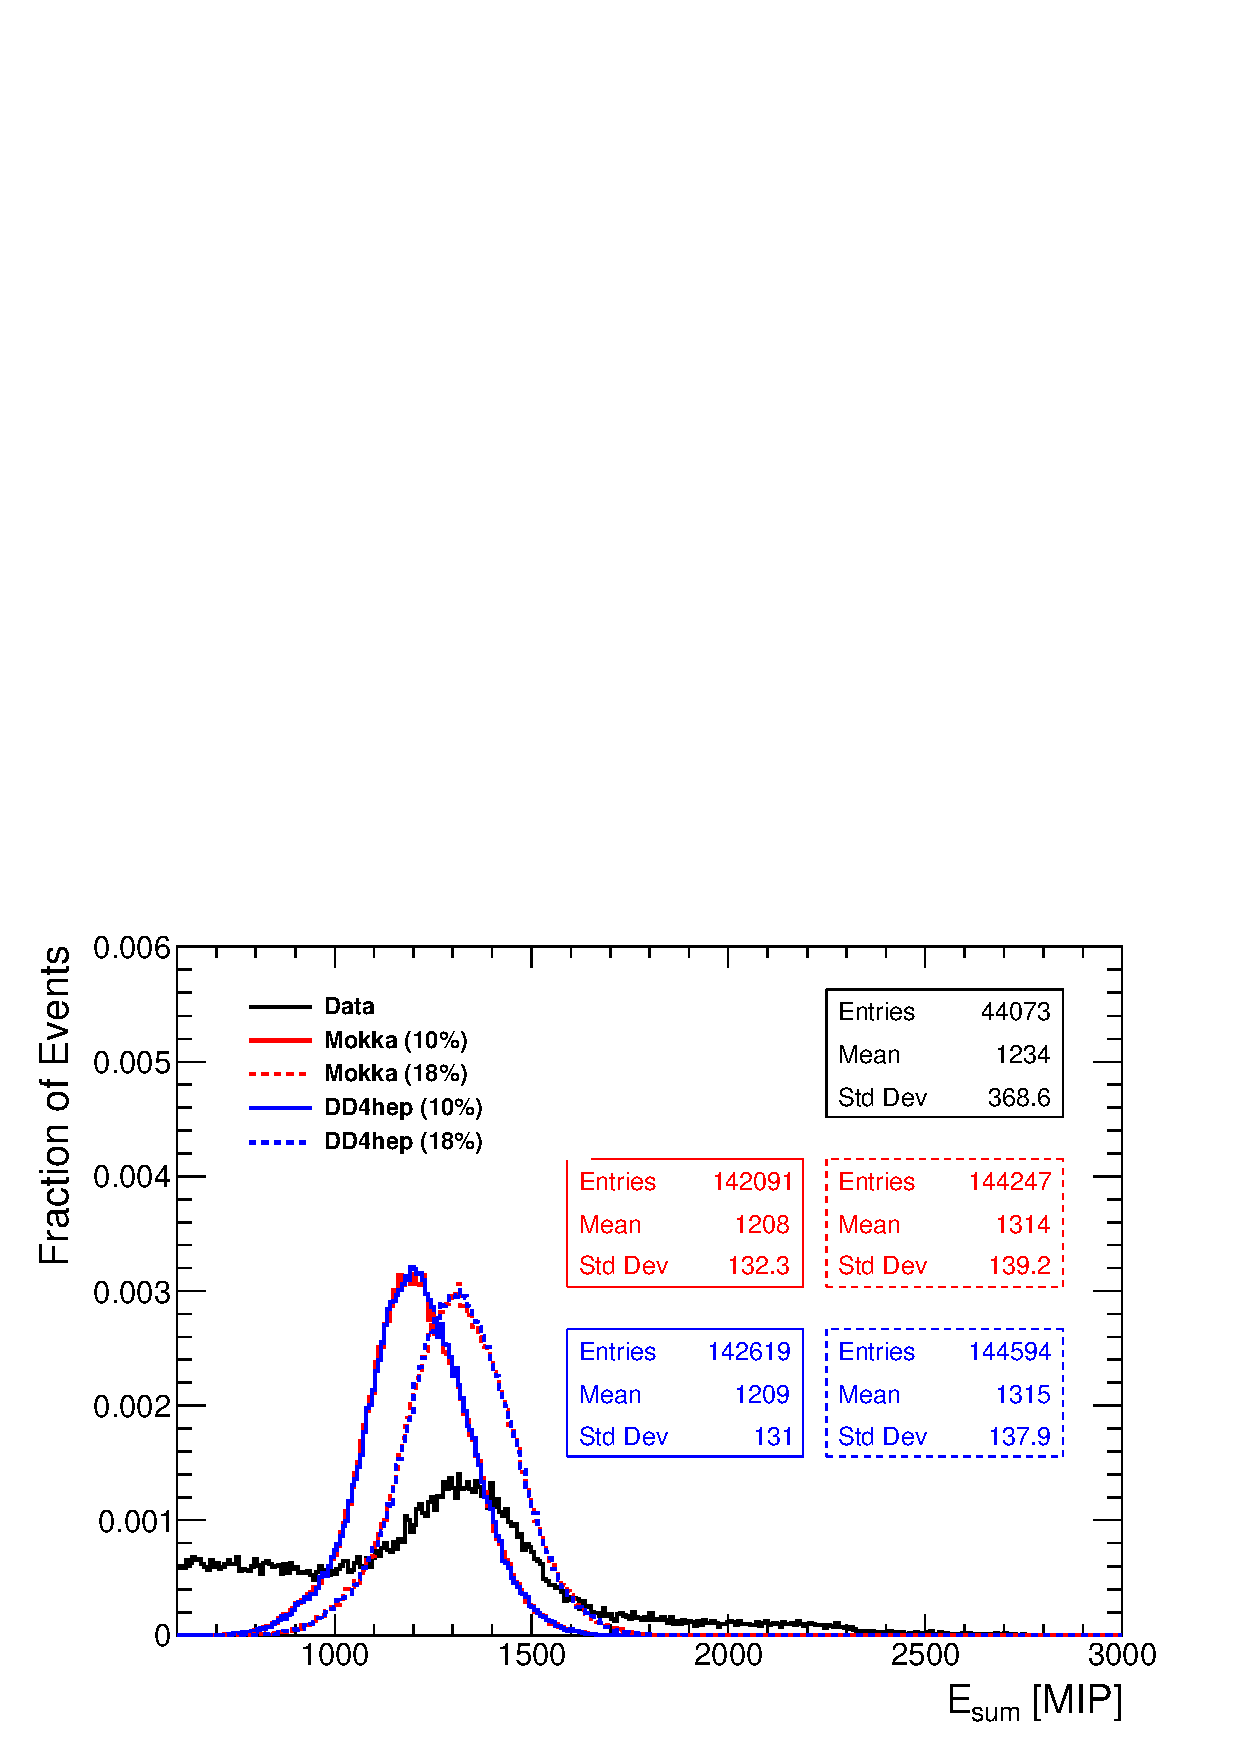
\includegraphics[width=1.\linewidth]{../Thesis_Plots/Timing/Electrons/Plots/Comparison_EnergySum_Xtalk_electrons50GeV.pdf}
    \caption{$E_{sum}$.} \label{fig:e50Evis}
  \end{subfigure}
  \hfill
  \begin{subfigure}[t]{0.49\textwidth}
    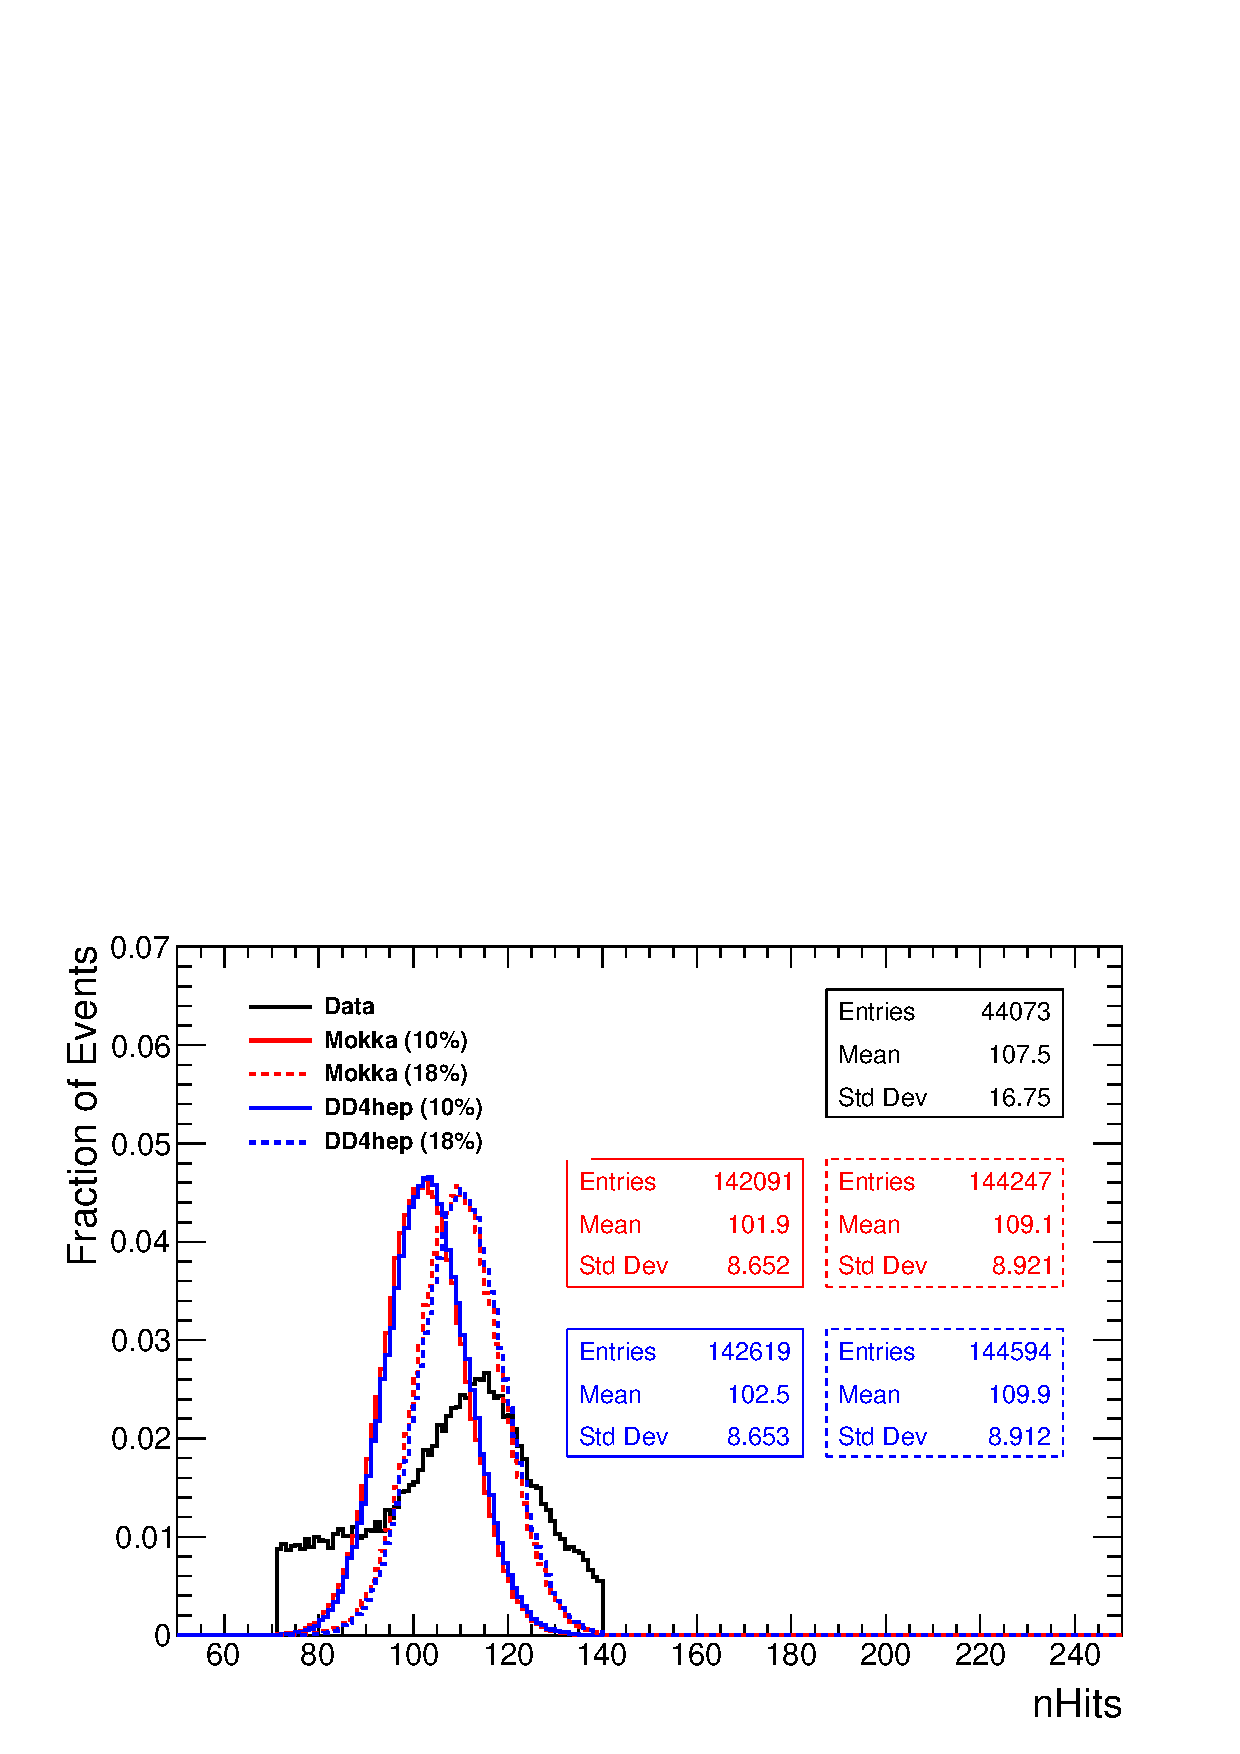
\includegraphics[width=1.\linewidth]{../Thesis_Plots/Timing/Electrons/Plots/Comparison_nHits_Xtalk_electrons50GeV.pdf}
    \caption{nHits.} \label{fig:e50nHits}
  \end{subfigure}
  \caption{\subref{fig:e50Evis}) The energy sum in the AHCAL for 50 GeV electrons for data and simulations with a cross-talk value of 10\% and 18\%. \subref{fig:e50nHits}) The number of hits in the AHCAL for 50 GeV electrons for data and simulations with a cross-talk value of 10\% and 18\%.}
  \label{fig:e50Val}
\end{figure}

Figures \ref{fig:eVal} show the mean energy sum $<E_{sum}>$ and the mean number of hits $<nHits>$ as function of the electron beam energy between 10 and 50 GeV for data and simulation with different cross-talk parameters. The visible energy for data agrees within the simulations for 10, 15 and 20 GeV electron energy and seems to agree better with the 10\% cross-talk simulations. For higher energies, the data deviates significantly to lower values due to the presence of the long tail left of the distribution that the simulations cannot describe. The number of hits is well described, certainly due to the selection cut on the number of hits, with the simulations but agrees better with 10\% at low energies and with the 18\% at higher energies. However, the data cannot be described for both distributions at once in either simulation with a global cross-talk parameter.

\begin{figure}[htbp!]
  \centering
  \begin{subfigure}[t]{0.49\textwidth}
    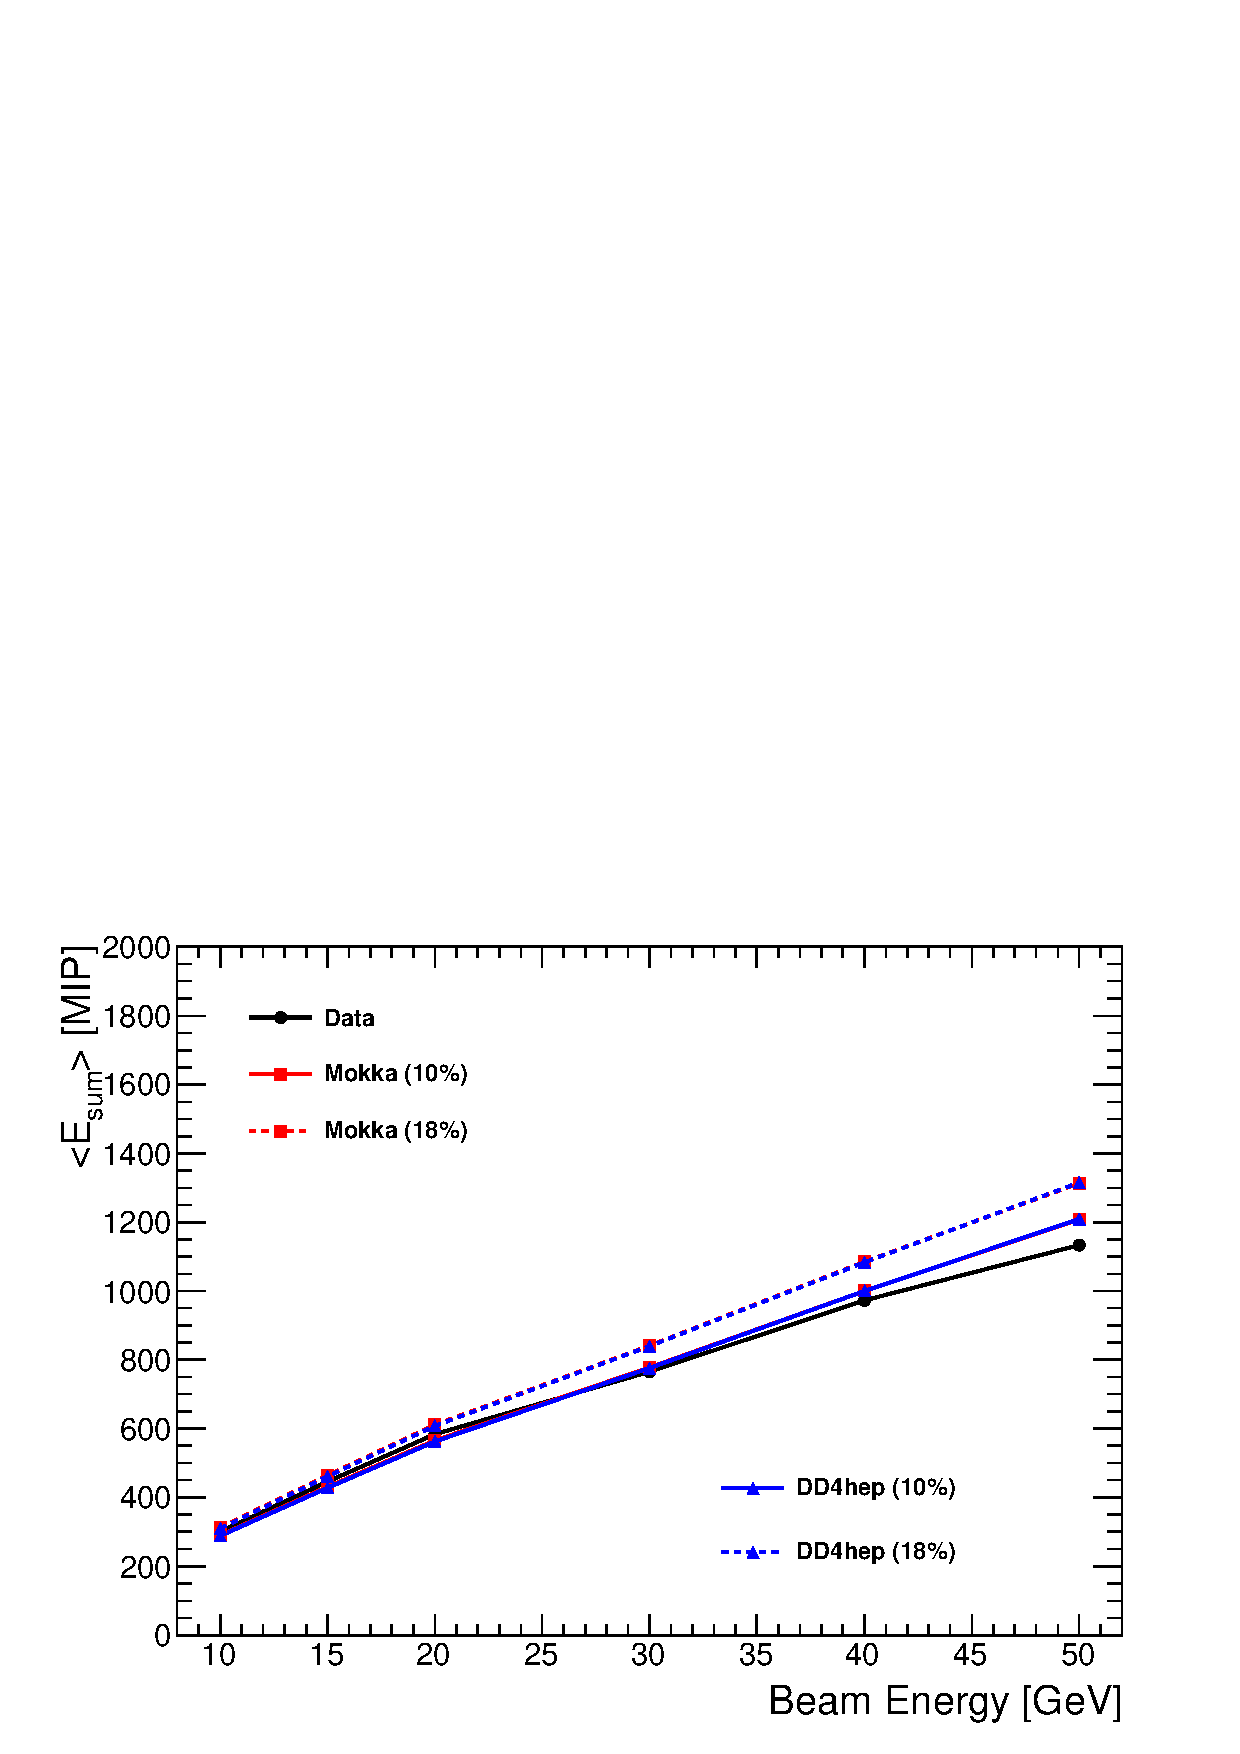
\includegraphics[width=1.\linewidth]{../Thesis_Plots/Timing/Electrons/Plots/EsumElectrons_BeamEnergy.pdf}
    \caption{} \label{fig:EsumMeanElectron}
  \end{subfigure}
  \hfill
  \begin{subfigure}[t]{0.49\textwidth}
    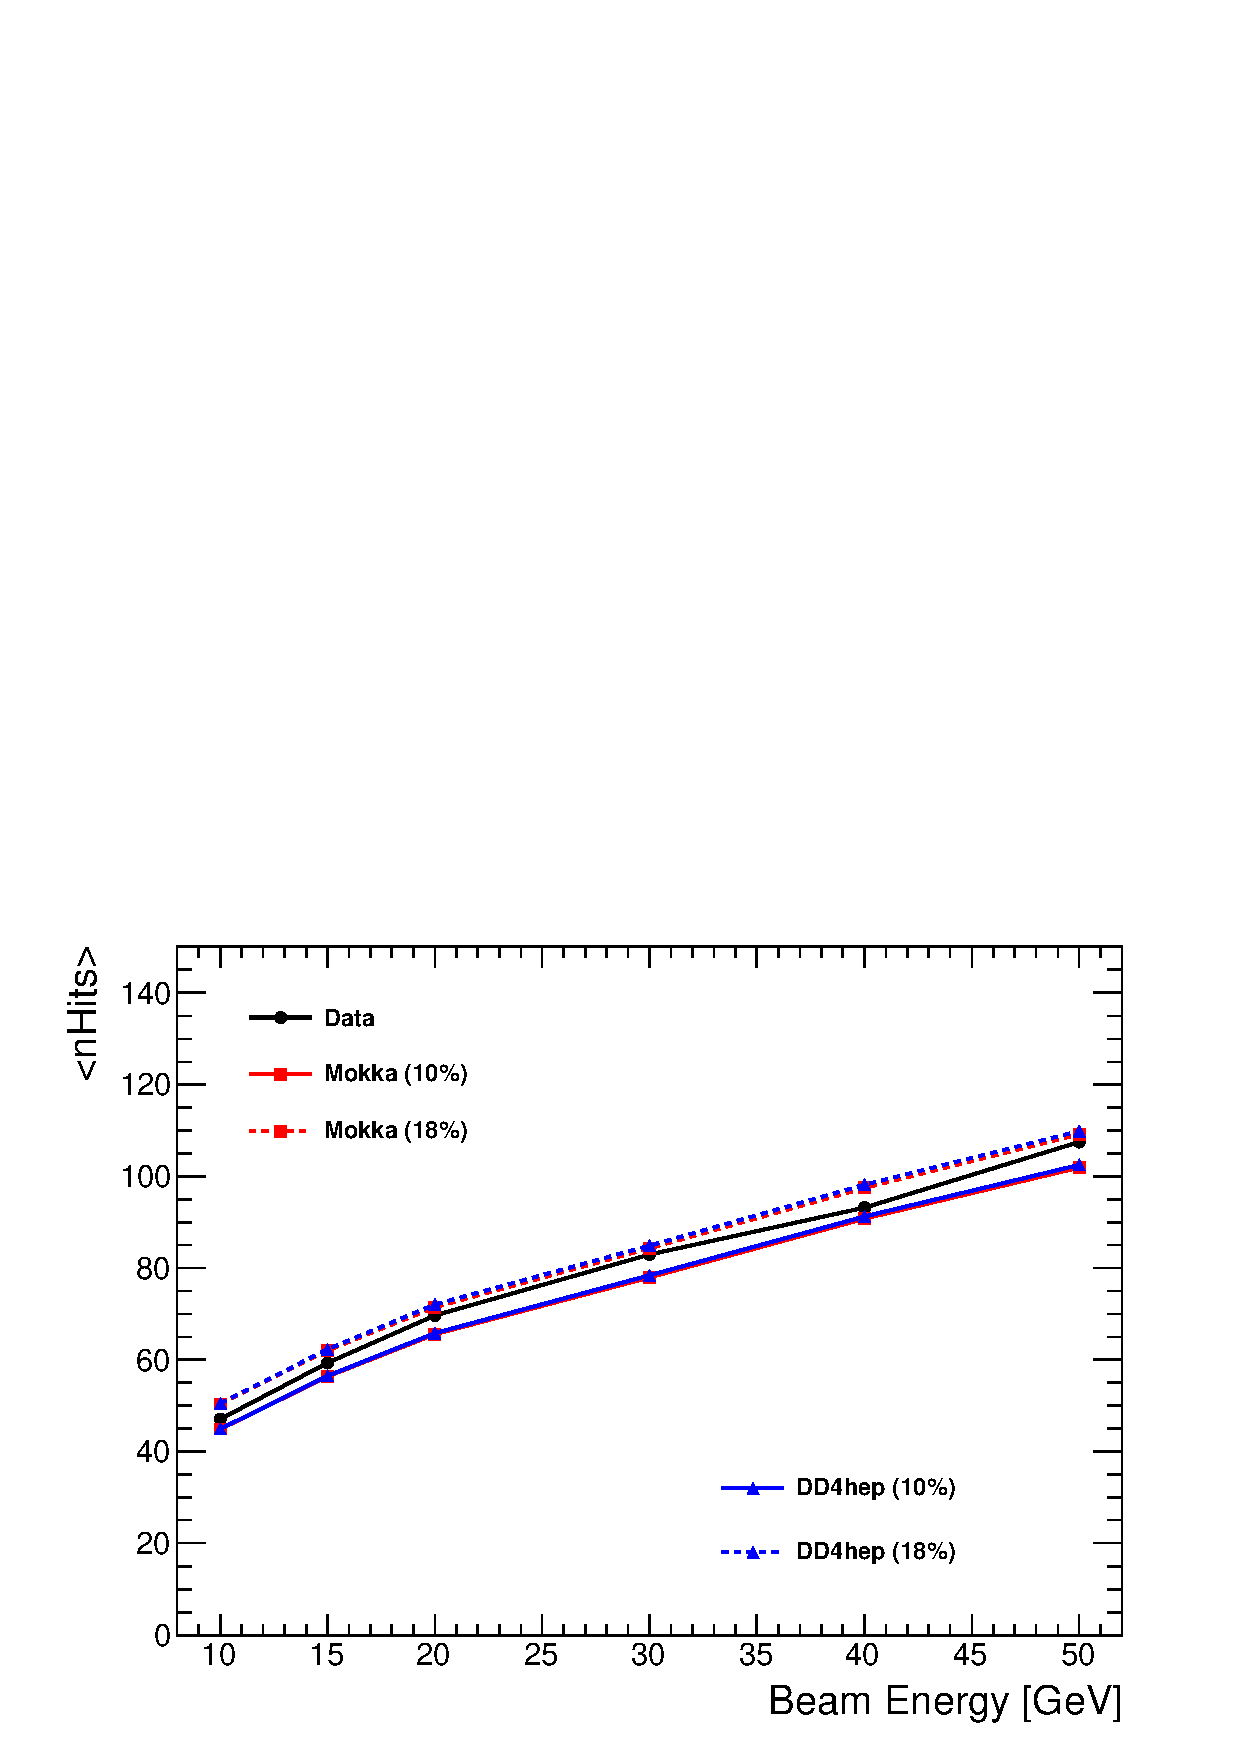
\includegraphics[width=1.\linewidth]{../Thesis_Plots/Timing/Electrons/Plots/nHitsElectrons_BeamEnergy.pdf}
    \caption{} \label{fig:nHitsMeanElectron}
  \end{subfigure}
  \caption{\subref{fig:EsumMeanElectron}) Comparison of the mean energy sum in the AHCAL as function of the beam energy for electron data and simulations with different cross-talk parameters. \subref{fig:nHitsMeanElectron}) Comparison of the mean number of hits in the AHCAL as function of the beam energy for electron data and simulations with different cross-talk parameters.}
  \label{fig:eVal}
\end{figure}

The investigation of these observables enables us to validate the simulations between 5-20\% with the data. The precision of the detector simulation for electrons is limited by the cross-talk simulation and for energies above 20 GeV, by the possible contamination by low energy electrons in the data. A deeper investigation on the energy aspect of the data is carried out in parallel of this analysis \cite{AmbraEnergy}.

\subsection{Pions}

Finally, the pion data was compared to simulations. In this case, the QGSP\_BERT\_HP physics list was only used for comparison. The center of gravity in the z-direction, the number of hits and the energy sum are the variables looked at and are shown in figures \ref{fig:piGoGZ}, figures \ref{fig:pi10Val} and figures \ref{fig:pi90Val}.

\begin{figure}[htbp!]
  \centering
  \begin{subfigure}[t]{0.49\textwidth}
    \includegraphics[width=1.\linewidth]{../Thesis_Plots/Timing/Pions/Plots/Comparison_CoGZ_Xtalk_pions10GeV.pdf}
    \caption{$CoGZ$ 10 GeV.} \label{fig:pi10CoGZ}
  \end{subfigure}
  \hfill
  \begin{subfigure}[t]{0.49\textwidth}
    \includegraphics[width=1.\linewidth]{../Thesis_Plots/Timing/Pions/Plots/Comparison_CoGZ_Xtalk_pions90GeV.pdf}
    \caption{$CoGZ$ 90 GeV.} \label{fig:pi90CoGZ}
  \end{subfigure}
  \caption{Distributions of the center of gravity in the z direction for data and simulations of 10 GeV (left) and 90 GeV (right) pions. The simulations have a cross-talk value of 10\% and 18\%.}
  \label{fig:piGoGZ}
\end{figure}

In figure \ref{fig:piGoGZ}, for 10 GeV pions, the CoGZ is well reproduced by the simulations with a cross-talk value between 10\% and 18\% whereas, for 90 GeV pions, small discrepancies are visible between data and simulations. Also, it is noticeable that the \ddhep and \mokka simulations also differ slightly. The reason is not clear. The discrepancy with the data may be related to multi-particle events as shown in the figures below.

The figure \ref{fig:pi10Val} shows the comparison between data and simulation with cross-talk values of 10\% and 18\% of the energy sum and number of hits distributions for 10 GeV pions. The data is well reproduced by the simulations. The figure \ref{fig:pi90Val} shows the same distributions for 90 GeV pions. Some discrepancies are visible between data and simulations, especially for the energy sum where a second peak is visible in data and may be from multi-particle events. A slight shift for the first peak is visible and may come from mis-calibrations (intercalibration of high/low gain). Concerning the number of hits, the \mokka simulation represents well the data as for \ddhep it over-estimates the fraction of events around 40-50 hits and under-estimates it over 80 hits.

\begin{figure}[htbp!]
  \centering
  \begin{subfigure}[t]{0.49\textwidth}
    \includegraphics[width=1.\linewidth]{../Thesis_Plots/Timing/Pions/Plots/Comparison_EnergySum_Xtalk_pions10GeV.pdf}
    \caption{$E_{sum}$.} \label{fig:pi10Evis}
  \end{subfigure}
  \hfill
  \begin{subfigure}[t]{0.49\textwidth}
    \includegraphics[width=1.\linewidth]{../Thesis_Plots/Timing/Pions/Plots/Comparison_nHits_Xtalk_pions10GeV.pdf}
    \caption{nHits.} \label{fig:pi10nHits}
  \end{subfigure}
  \caption{\subref{fig:pi10Evis}) The energy sum in the AHCAL for 10 GeV pions for data and simulations with a cross-talk value of 10\% and 18\%. \subref{fig:pi10nHits}) The number of hits in the AHCAL for 10 GeV pions for data and simulations with a cross-talk value of 10\% and 18\%.}
  \label{fig:pi10Val}
\end{figure}

\begin{figure}[htbp!]
  \centering
  \begin{subfigure}[t]{0.49\textwidth}
    \includegraphics[width=1.\linewidth]{../Thesis_Plots/Timing/Pions/Plots/Comparison_EnergySum_Xtalk_pions90GeV.pdf}
    \caption{$E_{sum}$.} \label{fig:pi90Evis}
  \end{subfigure}
  \hfill
  \begin{subfigure}[t]{0.49\textwidth}
    \includegraphics[width=1.\linewidth]{../Thesis_Plots/Timing/Pions/Plots/Comparison_nHits_Xtalk_pions90GeV.pdf}
    \caption{nHits.} \label{fig:pi90nHits}
  \end{subfigure}
  \caption{\subref{fig:pi90Evis}) The energy sum in the AHCAL for 90 GeV pions for data and simulations with a cross-talk value of 10\% and 18\%. \subref{fig:pi90nHits}) The number of hits in the AHCAL for 90 GeV pions for data and simulations with a cross-talk value of 10\% and 18\%.}
  \label{fig:pi90Val}
\end{figure}

Finally, the mean energy sum $<E_{sum}>$ and the mean number of hits $<nHits>$ as function of the beam energy between 10 and 90 GeV for data and simulation with different cross-talk parameters were looked at as for electrons and are shown in figure \ref{fig:piVal}. The visible energy for data is above the simulations for all energies but agrees better with simulations for 10 and 50 GeV points. For higher energies, the data deviates significantly to higher values that may be due to multiple particle events shifting the mean of the distribution to higher energy values. The number of hits is well described by the \mokka simulation and slightly lower for the \ddhep simulation that is also visible in the mean energy sum. The reason is not clear as the material description is very similar in both simulations as shown with electrons.

\begin{figure}[htbp!]
  \centering
  \begin{subfigure}[t]{0.49\textwidth}
    \includegraphics[width=1.\linewidth]{../Thesis_Plots/Timing/Pions/Plots/EsumPions_BeamEnergy.pdf}
    \caption{} \label{fig:EsumMeanPion}
  \end{subfigure}
  \hfill
  \begin{subfigure}[t]{0.49\textwidth}
    \includegraphics[width=1.\linewidth]{../Thesis_Plots/Timing/Pions/Plots/nHitsPions_BeamEnergy.pdf}
    \caption{} \label{fig:nHitsMeanPion}
  \end{subfigure}
  \caption{\subref{fig:EsumMeanPion}) Comparison of the mean energy sum in the AHCAL as function of the beam energy for pion data and simulations with different cross-talk parameters. \subref{fig:nHitsMeanPion}) Comparison of the mean number of hits in the AHCAL as function of the beam energy for pion data and simulations with different cross-talk parameters.}
  \label{fig:piVal}
\end{figure}

In conclusion, the investigation of these observables for pions enables us to validate the simulations between 10-20\% with the data. The precision of the detector simulation for pions is limited by the cross-talk simulation and by the possible contamination by multi-particle events in the data.

\begin{center}
  \rule{0.5\textwidth}{.4pt}
\end{center}

This chapter presents the results of the energy scale calibration of the AHCAL technological prototype. The MIP calibration procedure was explained and developed in order to accommodate to such high number of channels as well as the diversity in SiPM types and tile designs. In this way, 85\% of the channels in the detector have their MIP constant determined.

An error around 1-3\% is made on the MIP constant value with the current fitting method which is in the order of magnitude expected due to the limited statistics. In order to validate the calibration and the simulation model, comparisons have been made at the single channel level. Both data and simulation are in a good agreement with less than 1\% deviation. The simulation appears narrower due to channel-wise mis-calibrations not being modeled. A systematic uncertainty of 3.6\% on the MIP energy scale has been determined due to run-by-run, time and environmental variations.

An extensive validation of the simulation has been done and proves to be reliable between 10\% to 20\% with the data. As the simulation is validated, the timing study of hadronic shower which is at the core of this thesis can be studied. Before studying the time development of hadron shower, the time of a hit recorded in data needs to be calibrated. Therefore, in the next chapter, the timing calibration of the AHCAL prototype is presented.
